\documentclass[peerreview]{ieeesyscoin}
\usepackage{cite}
\usepackage{amsmath,amssymb,amsfonts}
\usepackage{algorithmic}
\usepackage{enumitem}
\usepackage{caption}
\usepackage{xcolor}
\usepackage{graphicx}
\usepackage{textcomp}
\usepackage{multirow}
\usepackage[switch]{lineno}
\def\BibTeX{{\rm B\kern-.05em{\sc i\kern-.025em b}\kern-.08em
    T\kern-.1667em\lower.7ex\hbox{E}\kern-.125emX}}
\begin{document}

\history{}

\title{\centering Syscoin 4: A Peer-to-Peer Electronic Cash System Built For Decentralized
Web 3.0 Business Applications}
\author{\centering  \uppercase{Jagdeep Sidhu, MSc}\authorrefmark{1}, 
and \uppercase{Ian C. Moore, PhD\authorrefmark{2}}}

\address[1]{\centering Syscoin Core Developer, Blockchain Foundry Inc.(e-mail: jsidhu@blockchainfoundry.co)}
\address[2]{\centering  (Syscoin Researcher, e-mail: imoore@syscoin.org)}
\tfootnote{}

\markboth
{Sidhu \headeretal: Syscoin 4: A Peer-to-Peer Electronic Cash System Built For Decentralized
Web 3.0 Business Applications}
{Sidhu \headeretal: Syscoin 4: A Peer-to-Peer Electronic Cash System Built For Decentralized Web 3.0 Business Applications}

\corresp{}

\begin{abstract}
Syscoin 4 introduces a novel implementation of a UTXO Asset platform with instant, pseudo-interactive, zero-confirmation, double-spend protected cryptocurrency transactions (Z-DAG) as well as an EVM, both secured via Nakamoto Consensus PoW through merged-mining with Bitcoin. Masternodes providing bonded validators with chainlocks help to reduce selfish-mining opportunities as well as provide the network with full node security. The EVM scales on layer 2 with Zero-Knowledge Proofs and the UTXO Asset platform scales on layer 2 with payment channels.
\end{abstract}

\begin{keywords}
Network EVM, DAG, Decentralized Identity, Zero-Knowledge Proofs, UTXO, Assets, Layer 2, Web3
\end{keywords}

\titlepgskip=-15pt

\maketitle

\section{Introduction}
\label{sec:introduction}

Syscoin 4 builds on Syscoin 3 with the additional implementation of an Ethereum Bridge, Offers/Escrow, Lightning Network, and Decentralized Identity. As previously featured \cite{Sida18}, anything pertaining to the Marketplace (e.g., digital sales, auctions, marketplace modification, etc.) has been deprecated. The full release will include the Syscoin Network-Enhanced Virtual Machine (NEVM), which will utilize the Ethereum Virtual Machine (EVM) coupled with a Zero-Knowledge Proof (ZKP) system to build scalable applications, and the introduction of a decentralized cost model around Ethereum Gas fees (see Table \ref{table:ugrades}).

High gas fees and low transaction throughput are some of the key issues that are hindering ERC-20 projects from running at scale. Ethereum 2.0 is currently under development to address these issues. However, its final release is not anticipated to be completed for several years \cite{But19}. Instead of building a competing smart contract system, we have decided to work with the EVM protocol to build a faster, cost effective, alternative to Ethereum 2.0. To achieve this, the roadmap for Syscoin 4 proposes a four-layer tech-stack \cite{Sig21} comprised of: (a) Syscoin as the base layer to provide security; (b) EVM for programmability; (c) ZKP for scalability; and (d) applications to provide decentralized usability for the next phase of the internet's evolution, known as Web 3.0. 

In Section \ref{sec:protocol} we address the protocol attributes, which include Z-DAG, order-of-events, point-of-sale applications, assets, non-fungible tokens, Lightning Networks, offers/escrow, and masternodes. In Section \ref{section:roadmap} we lay out the roadmap for Syscoin 4, which includes scalability, design proposal, performance evidence, and applications. In Section \ref{section:specs} we outline the protocol specifications, and conclude the article in Section \ref{section:summary}.

\begin{table}[h!]
\caption{Syscoin 4 Upgrades and Modifications}
\label{table:ugrades}
\setlength{\tabcolsep}{3pt}
\begin{tabular}{|p{135pt}|p{75pt}|}
\hline
Syscoin Feature & 
Update \\

\hline
Nakamoto ZDAG (ie, Z-Dag) & no change \\
Assets & modified \\

Offers and decentralized marketplace &   \\
~~~~~ Digital Sales &  deprecated \\
~~~~~ Auctions &  deprecated \\
~~~~~ Reselling w/ whitelists &  deprecated \\
~~~~~ Feedback and rating &  deprecated \\
~~~~~ Multiple payment options &  deprecated \\
~~~~~ Shipping notification system &  deprecated \\
~~~~~ Marketplace moderation &  deprecated \\

Data Anchoring &  deprecated \\
Instant Encrypted Messages &  re-purposed \\
Blockchain pruning &  deprecated \\
Certificates (see Identity) &  modified \\
Decentralized Identity &  new feature \\
~~~~~ Certificates &  modified \\
Lightning networks &  new feature \\
Offers / Escrow &  modified \\
Roadmap to Web 3.0 & \\
~~~~~ Network EVM (NEVM) &  new feature  \\
~~~~~ Zero Knowledge Proofs &  new feature \\
~~~~~ NEVM Applications &  proposed \\

\hline
\multicolumn{2}{p{251pt}}{depreciated  $\rightarrow$ removed from Syscoin 4; modified  $\rightarrow$ repurposed from Syscoin 3; new feature  $\rightarrow$ upgrade from Syscoin 3; no update $\rightarrow$ carry-over from Syscoin 3}\\

\end{tabular}
\label{tab1}
\end{table}


\section{Protocol Characteristics}
\label{sec:protocol}

\subsection{Z-DAG}
Zero-Confirmation Directed Acyclic Graph (Z-DAG) is an instant settlement protocol functioning across all Syscoin services. Syscoin services consist of Alias Identities, Certificates, Escrow, Offers and Assets. Each service is controlled via an Alias, in which ownership is proven through a private key that matches each
unique address. Z-DAG organizes transactions based on dependencies to build the state in a deterministic fashion. This helps protect against double-spends where an asset is transferred falsely by creating multiple transactions through multiple nodes within a short time \cite{Sida18}.

\begin{figure}[h!]
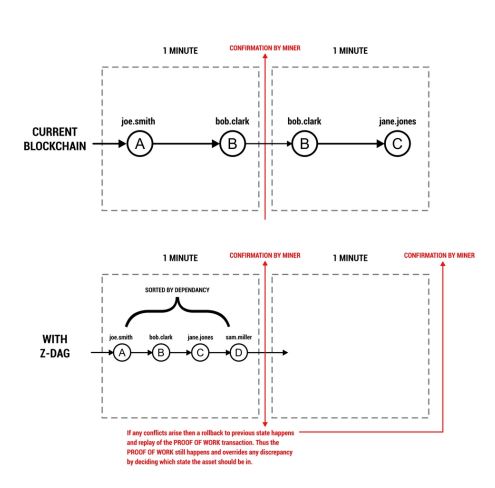
\includegraphics[width=3in]{img/current_vs_zdag.png}
\caption{Current Blockchain design vs Z-DAG} 
\label{fig:current_vs_zdag}
\end{figure} 

Figure \ref{fig:current_vs_zdag}  shows the difference between a regular blockchain and Syscoin’s Z-DAG implementation. Syscoin now has two consensus layers. The upper layer consists of a Z-DAG graph of transactions are represented in the mempool without a block, providing settlement in real-time. The lower layer provides confirmation and conflict resolution preventing double-spend events through existing Proof-of-Work (PoW) consensus.

When verifying, client nodes will create a graph of transactions topologically arranged via ascendants and descendants organized by the asset UTXO being spent. This is the most efficient approach as a circuit detection is not required; rather, it is inherently assumed as it is added to coin indexes in the memory pool.

Z-DAG is a transactional algorithm and does not affect consensus policy. It is meant to be a double-spend detection and prevention algorithm through the transaction policies of Syscoin Core.

A User Interface (UI) layer will notify the user of conflicts in real-time, allowing the transaction to occur in 3 to 5 seconds (i.e., the amount of time the network takes to notice that 2 double-spend transactions are conflicting with each other). This is possible through Syscoin’s Masternode layer that consists of incentivized full nodes paid an allocation of subsidy every block. Every masternode is connected to 25 or more peers, which facilitates high-throughput relay across the network, averaging one or more network hops to transmit from the sender to the receiver nodes.

To accurately detect double-spends, other implementations such as Phantom \cite{Som18} or Spectre \cite{Som15} must replace the longest chain rule to derive the order of events and attacker sequences in a graph.
These implementations end up in a more complex game theoretical situation that has not  been proven mathematically to be accurate in all cases. Syscoin relies on the thoroughly tested Nakamoto consensus model to arrive at a consensus over time rather than simply relying on a DAG.

\subsection{Order-of-events preservation and Conflict Resolution}
Since assets have been migrated to a UTXO model in Syscoin 4, order-of-events and conflict resolution is as simple as relying on the existing UTXO policy of the Bitcoin memory pool code, which orders individual UTXO dependencies as ascendants and descendants per output. The conflict resolution code for double-spending an output was slightly adjusted from the Bitcoin policy by allowing one double-spend attempt for each output to propagate across the network. This ensures that a double-spend will always be detectable by an observer regardless of order-of-events. This is especially important as nodes on the network have no ability to understand the intent of a transaction and are thus not able to know which one is actually a double-spend attempt. To account for the extra bandwidth requirements of allowing a double-spend to be propagated, the minimum relay fee paid in the transaction is double that of a regular transaction. 


\subsection{CAP Theorem}
The CAP theorem \cite{Bre12} states that it is impossible for a distributed data store to simultaneously provide more than two out of the following three guarantees: consistency, availability or partition tolerance. Bitcoin attempts to provide a guarantee that transactions are settled, but is not able to do so according to theory. Z-DAG partially trades consistency for availability. Since it is unlikely that a double-spend or re-organization will change the state of someone’s balance, we do not wait for settlement finality by waiting for blocks to confirm. This drastically increases the usability in point-of-sale applications.

The allowance of instant settlements and increased availability requires paying additional attention to users simply trying to double-spend or send transactions too quickly, which may cause the miner view to change from the general network view. The DAG will order the dependency graph of transactions and process in sequence, allowing for better availability (i.e., client making a request for data gets a response) when it comes to instant state changes. The same CAP constraints as PoW will provide a more responsive money transfer mechanism that may be used as a transaction processor instead of simply a settlement layer.

\subsection{Point-of-sale applications}
The combination of using assets with Z-DAG will allow for point-of-sale applications, providing real-time exchange of cryptocurrency assets/tokens.

\subsection{Assets}
We have created a coloured-coin implementation of a UTXO asset model where the commitment to the specific values of the assets are embedded in OPRETURN data carrying payload. The UTXO itself is part of the transaction to keep compatibility with the Bitcoin transaction format. The consensus to prove validity of an asset transaction is to simply compare the map of inputs (pairing of asset GUID and total value across all inputs) and the map of all outputs (pairing of asset GUID and total value across all outputs), which must be equal (note: there is no fee on assets so equality is sufficient to ensure validity). The coin database storing the unspent outputs adds a value to represent the asset identifier (GUID) for asset outputs.

\subsection{Non-Fungible Tokens}

Non-Fungible Tokens (NFTs) are unique Syscoin-based digital assets.  Some potential use cases include: gaming, digital art, physical assets, and digital collectibles. The advantages of using Syscoin over other platforms include, but is not limited to scalability, divisibility, efficiency, and notary capabilities. 

By utilizing the NEVM, Syscoin will offer NFTs running on the application layer of its tech-stack, which will offer a competitive advantage over Ethereum in terms of scalability. Another interesting feature Syscoin will offer is divisibility. A good example of this is land ownership where fractions of such assets can be apportioned between multiple parties. Finally, developers will be able to employ notary capabilities by applying custom rule sets to transactions involving NFTs.

NFT, fractional or otherwise, are implemented in the UTXO asset model and of course can be deployed using the ERC-related specifications on the NEVM model as is the case with Ethereum. Notary capabilities are only implemented for the UTXO asset model. However, with validity proofs we are looking to integrate such features on the NEVM model as well.

\subsection{Decentralized Identity}
Decentralized Identity is the cornerstone for secure information and value exchange between people and devices. Typically current implementations leverage Hyperledger Aries to build Identity solutions following the Web3 RFC spec for Decentralized Identifiers (DID's) \cite{DID}. Through the use of public permission settlement of state, and zero-knowledge-proof based validity proofs to attest identity information (i.e., birth certificate or college diploma), we believe this is an ideal solution, which will not only scale to multiple jurisdictions needing to rely on identities issues by governments, but also allow for applications utilizing  social proof-of-person. Scaling is a challenge not only for privacy chains but also private-permissioned blockchains (the registrations of identities are not aggregated and put onto the ledger on a FIFO basis) There is also the issue that settlement happens not on public infrastructure but private and so is susceptible to attacks, which casts doubts over the claim of immutability. Built on zkRollup infrastructure, identity systems can not only scale, but data can remain private and settlement of state can be done on public infrastructure. We leave specific implementations up to integrators and enterprises looking to build next-generation identity solutions.

\subsubsection{Selfish mining}

Selfish mining is a long standing open problem in the Bitcoin ecosystem \cite{Eya18}. However, with the introduction of masternodes and the ChainLocks service, we have innovated a mechanism design that falls back to Nakamoto consensus. Yet, if a chain lock in a block exists will remove selfish mining attack vectors. To understand the solution it is important to understand the design of Multi-quorum based Chain locks.

\subsubsection{Chain locks}

With a subset of nodes offering sybil resistance through the requirement of bonding 100,000 SYS to become active, along with the deterministic masternode feature added in Syscoin 4.2, we have enabled Chain Locks to prevent selfish mining. Dashcore was the first project to implement this idea \cite{Blo18}, which the industry has since widely accepted as a viable solution \cite{Val19}. Our implementation is a simplified and optimized version of the original. We do not implement Instant Send or Private Send transactions. Due to Syscoin being merged-mined with Bitcoin, we believe our chain coupled with Chain Locks becomes more secure via solving Bitcoin’s most vulnerable attack vector (i.e., selfish mining). 

Chain Locks are made part of Long-Living Quorums (LLMQ) which leverage aggregatable Boneh–Lynn–Shacham (BLS) signatures that have the property of being able to combine multiple signers in a Distributed Key Generation (DKG) event to sign on decisions. In this setup, a signature can be signed on a group of parties under threshold constraints without any one of those parties holding the private key associated with that signature. In our case, the signed messages would be a ChainLock Signature (CLSIG) which represent claims on what block hashes represent on the canonical chain \cite{Blo18}. This model suggests a very efficient   threshold signature design was needed to reach consensus across the Masternode layer, decide on chain tips, and lock chains, hence preventing selfish mining attacks. See \cite{Bon18} to understand the qualities of BLS signatures in the context of multi-signature use cases.

Ethereum 2.0 caters to the use of BLS signatures through adding precompile opcodes in the Ethereum Virtual Machine (EVM) for the BLS12-381 curve \cite{Dra18}, which Syscoin has adopted. This curve was first introduced in 2017 by Bowe \cite{Bow17}  to the ZCash protocol. Masternodes on Syscoin have adopted this curve and have a BLS key that is associated with each validator. See \cite{Blo18} for performance comparison to ECDSA (Secp256k1) and a discussion on usefulness in contrast to what Bitcoin and Syscoin natively use for signature verification.


\subsection{Lightning Networks}
By extending on the UTXO asset model we look to integrate layer 1 assets into transactions on layer 2 payment channels such as Lightning Networks \cite{Poon16}. Adding multiple assets to LN requires solving theoretical attack vectors related to American call-options as described in \cite{LN}. Since Syscoin UTXO assets enable the transacting of multiple assets in a single transaction, the integration into Lightning Networks should be fairly intuitive once the problems related to American call-options are solved for.

\subsection{Masternodes}

With 2500+ current, active masternodes running fullnodes, Z-DAG becomes more dependable, as does the propagation of blocks and potential forks. Masternodes are bonded through a loss-less strategy of putting 100,000 syscoin in an output and running full nodes in exchange for block rewards. A seniority model incentivizes masternodes to share long-term growth by paying more for the longer period of service as an additional incentive. Half of the transaction fees are shared between the PoW miners and masternodes to ensure long-term alignment once block subsidy becomes negligible. Coins are not locked at any point, and there is no slashing condition if masternode owners decide to move their coins, the rewards to those masternodes simply stop. Sharing Bitcoin’s compact block design, it consumes very little bandwidth to propagate blocks assuming the memory pool of all these nodes is roughly synchronized \cite{BitCore}. The traffic on the network primarily consists of propagating the missing transactions to validate these blocks. Having a baseline for a large number of full nodes that are paid to be running allows us to create a very secure environment for users. It proposes higher costs to would-be attackers who either have to attempt a 51\% attack on Syscoin (i.e., effectively trying to attack the Bitcoin network), or try to game the mesh network by propagating bad information which is made more difficult by incentivized full nodes. The health of a decentralized network relies on the following; (a) the mining component, or consensus to produce blocks, and (b) the network topology to disseminate information in a timely manner in conditions where adversaries might be lurking. The likelihood of other attacks related to race conditions in networking or consensus code are minimized by following a rigorous, thorough and continuous development process. This includes deterministic builds, Fuzz tests, ASAN/MSAN/TSAN, functional/unit tests, multiple clients and adequate code coverage. Syscoin and Bitcoin protocol code bases are merged daily such that the build/signing/test processes are all identical, allowing us to leverage the massive developer base of Bitcoin.  Code quality is reflective of taking worst-case situations into account. 

\section{Roadmap to Web 3.0}
\label{section:roadmap}

Bitcoin was the first to offer a practical solution to the General's Dilemma using Crypto Economic rationale and incentives. Ethereum was the first to abstract the concept of Turing completeness within similar frameworks assumed by Bitcoin. What Syscoin presents is a combination of both Bitcoin and Ethereum with intuitions built on top to achieve a more efficient financial computing platform that leverages coordination to achieve consensus using Crypto Economic rationale and incentives. We propose a four-layer tech stack using Syscoin as the base (host) layer, which provides an efficient (i.e., low gas cost per transaction) platform. Some of the main advantages include scalable, decentralized enabling applications, and the introduction of a decentralized cost model around Ethereum gas fees. This new model proposes state-less parallelized execution and verification models while taking advantage of the security offered by the Bitcoin protocol. 

\subsection{Scalability and Security}

Scalability in blockchain environments is typically measured by total Transactions per Second (TPS). This suggests full trustlessness, decentralization and liveness properties as evidenced by something like Bitcoin. If trade-offs are made to achieve higher scale, it means another property is affected. If two nodes are running the same hardware and doing the same work, the one that provides more TPS performance than the other is considered more scalable. This is not to be confused with throughput which is the measure of output that can be increased by simply adding more hardware resources. Hence, more throughput does not mean more scalable. Some blockchains require the producers of blocks to run on higher specifications, thus offering higher throughput but not necessarily scaling better. However, there are projects which employ parallel processing to try to achieve higher scale whilst also enforcing more capable hardware to provide a more efficient overall system [33]. As a logical experiment, the throughput of a system divided by the scalability of the system is what we define as efficiency. In the following sections, we will outline our proposal for improved efficiency.

\subsubsection{Efficiency}

The holy grail of blockchain design resides in the ability to have a ledger that can claim to be sublinear while retaining consistency, fault tolerance, and full availability (i.e., CAP Theorem). Hence, there are roughly constant costs for an arbitrary amount of computation performed and being secured by that ledger. Achieving this optimal tradeoff has always been thought of as impossible, unless acceptable trade-offs appear in application designs that are easy to understand. Most experts make the assumption that an O(1) ledger is simply impossible and thus design blockchains, and force applications, to work in particular ways as a result. We will remove such assumptions and let business processes dictate how they work by giving them the ability to achieve O(log kn) efficiency with trade-offs. A polylogarithmic design would give the ability for almost infinite scaling over time for all intents and purposes. The only bottleneck is the speed at which information can be propagated across the network. This in turn would improve over time as telecom infrastructure naturally evolves and increases in both capability and affordability.

Put in context, even Lightning Networks qualifies for transactional counts qualifies as a form of sublinear scaling on a TPS basis, but not per user as users must enter the main chain first before entering a payment channel. It requires the state of the blockchain to include users joining the system. This state (i.e., UTXO balances) is the primary  factor of efficiency degradation in Bitcoin. Users need to first start on the main chain and then move into the payment channel system to receive money, meaning that scale is at best O(N) where N is the number of users. There are some solutions to the problem of state storage on Bitcoin \cite{Dry19} (e.g., by reducing it via an alternative accumulator strategy to the cost of increased bandwidth). This approach would make the chain state-less. However, validation costs would remain linear in the number of transactions. When combined with payment channels, only costs to get in/out are factored into the validation. This offers an interesting design for payments themselves while providing for on-chain availability to help achieve scalable payments. Hence, it is not possible to employ that strategy with general computations. With this design we are still left with the issue of how to do general computations at higher efficiency.

What we present is the ability to have a polylogarithmic chain at the cost of availability for both payments and general computations, where business processes dictate availability policies and users fully understand the limitations of these policies when using such systems. Users will ensure availability for themselves and others at their discretion.  This will be expanded upon in the following sections.

\subsubsection{State Liveness and State Safety}

While many compelling arguments can be made migrating to a stateless design \cite{Hot19}, it is not possible to achieve sublinear efficiency without sacrificing some other desired component as outlined above. To achieve polylogarithmic efficiency, it is necessary to have a mix of stateless and stateless nodes working together in harmony on a shared ledger \cite{Hot19}. This should be accomplished so that business processes can dictate direction and users can choose to pay a little more for security, either by using a stateful (yet very scalable ledgering mechanism) or by paying to ensure their own data availability amortized over the life of that user on such systems. Presenting the ability for users to make these choices allows us to separate the consensus mechanism of such systems and reduce overall complexity. However, in whatever solution we adopt, we need to ensure that the final implementation allows for both the liveness and safety of that state. These are defined as follows:

\begin{itemize}
\item \textbf{State Liveness}: Transferring coins in a timely manner
\item \textbf{State Safety}:  Private custody
\end{itemize}

It is important to adhere to these concepts; unmoveable coins are worthless.

The options as described would allow users to decide their state liveliness at their own discretion, while state safety is a required constraint throughout any system design we provide. The doorway to possibilities of sublinear design is opened by giving users the ability to decide.


\subsubsection{Avoiding Re-execution of Transactions}

In order to scale arbitrarily, and independently of the number of transactions (a desired property of increasing throughput), one requires a mechanism to avoid re-executing transactions \cite{Bow18}; as these transactions put unnecessary additional overhead on the network. Ideally, it would be able to batch these transactions together for a two-fold scaling proposition. There are a few mechanisms in literature that attempted to solve re-execution: (a) TrueBit; (b) Plasma; and (c) Arbitrum avoided re-execution. Unfortunately, they require challenge response systems to ensure security, which leads to intricate attack vectors of unbounded risk/reward scenarios. 

Multi-Party Computation (MPC) is a mechanism that allows for shared computation while maintaining confidentiality and privacy. MPC is used in Syscoin for BLS threshold signatures for Chain Locks and Proof-of-Service in quorums of validators, deterministically chosen using Fiat-Shamir heuristics on recent block hashes. The problem with this approach is that validators may become corrupt, hence they need to be wrapped in a consensus system along with distributed key generation (DKG) and random deterministic selection. It was discarded due to the incentive for risk/reward scenarios to favour attacks as the value of the transactions increases.

Hardware enclaves (e.g., Intel SGX through remote attestation) were considered as a way to offload execution and avoid re-execution costs. 

ZKP allows for the desired superlinear scaling trait, but also offers other benefits - namely privacy is very easy to introduce and will not add detectable costs or complexity to verification on the mainchain. With users controlling their own data the mainchain and systems can be designed such that only balance adjustments are recorded, not transaction sets (we will explain the case with full data availability below). In this scenario there is no advantage for a miner to gain when colluding with users that launch attacks on systems such as Decentralize Finance (DeFi), pools and provenance of transactions. The flexibility has to be present for application developers that need experiences consistent with those we have today with Bitcoin/Syscoin/Ethereum. This would enable the privacy use-cases without requiring extra work, knowledge or costs.


\subsubsection{Validity Proof Systems Overtop Proof-of-Work Systems}

Prior to the use of Proof Systems, the only option for “Validity Proofs” in a permissionless system involved naive replay, which greatly limited scalability. Essentially, this is still practised in Layer-1 blockchain (L1) solutions, with the known penalty to scalability. Proof Systems offer a very appealing trait known as succinctness. How this works, in order to validate a state transition, one needs to only verify a proof, and this is done at a cost that is effectively independent of the size of the state transition (i.e., polylogarithmic in the size of the state transition).

For maximal financial security the amount of value being stored should depend on the amount of security provided on the settlement side of the ledger. PoW offers the highest security guarantees (see Appendix A). Our next generation financial systems begin with optimal ledgering security and add proof systems on top for scaling. Block times are not as important in a world where the majority of activity is on Layer-2 blockchain (L2) validity proof based systems. This liberates engineers, who are focused on scalability, to better define blocks, safe block times, as well as the maximal amount of data bandwidth that can be safely propagated in a time-sensitive manner across full nodes in the network. With Syscoin, there are incentivized full nodes (i.e., deterministic masternodes). So, again we can maximize the bandwidth of ledgering capabilities while retaining Bitcoin PoW security through merged-mining.


\subsubsection{Quantum Resistance}

Hashing with the SHA256 algorithm is regarded to be quantum safe because it requires Grover's algorithm to crack in the post-quantum world, and at best a quantum computer will offer a 50\% reduction in time to break \cite{Nai19}. On the other hand, where Shor’s algorithm applies, any pair based cryptographic system will be broken in hours.

For L2, we propose to implement ZKP in the SDK Layer; namely Non-Interactive Zero Knowledge Proofs (NIZKP). Popular implementations of NIZKP include Zero-Knowledge Succinct Non-interactive ARgument of Knowledge (zk-SNARKS) and Zero-Knowledge Scalable Transparent ARguments of Knowledge (zk-STARKS) \cite{Nas19}. There are some zk-STARK/zk-SNARK-friendly ciphers employed in zkRollup designs, such as MiMC and Pederson hashes, that would offer quantum resistance within ZKPs. However, we currently lack certainty on their classical security; despite this we are hopeful.

It is essential to acknowledge that Bitcoin was developed with change addresses in mind. Stealing Bitcoin requires exposing the hash of its public key, which can be done using Grover’s algorithm running on a quantum computer. Each time a Bitcoin Unspent Transaction Output (UTXO) is spent the public key is exposed and a new change address (which does not expose the public key) is used as change.

With this in mind, any scalable L2 solution should be quantum resistant because otherwise we undermine Bitcoin design as the gold standard of security.

\subsection{Design Proposal for Web 3.0}

The following describes the four layers (see Fig 2) of Syscoin’s proposed tech stack for Web 3.0:

\begin{enumerate}
\item \textbf{Host Layer:} Bitcoin’s design is the gold standard for security and decentralization. PoW and Nakamoto Consensus settlement security are widely regarded by academics as the most hardened solution for ledgering value \cite{Bit15}. However, it is also arguable that the intricate design encompassing Game Theory, Economics, risk reward ratios for attack, and the minimal amounts of compromising attack vectors is likely not to change for the foreseeable future. UTXOs (and payments with them) are more efficient than account-based or EVM-based solutions. That said, Bitcoin itself suffers from not being expressive enough to build abstraction for general computation. 
\item \textbf{Operating System Layer} EVM/eWASM is the gold standard for general computation because of its wide adoption in the community. Anyone building smart contracts is likely using this model, and will continue to use it as the standard for autonomous general computation with consensus.
\item \textbf{SDK Layer} Zero-knowledge proofs are the gold standard for generalized computation scaling for blockchain applications. They enable one-time execution via a prover and enable aggregated proof checking instead of re-execution of complex transactions via zk-STARKs or zk-SNARKs using collision resistant hash functions. At the moment generalized smart contracts are not there yet but we are quickly approaching the day (e.g., Cairo, Zinc) when there will be abstractions made to have most Solidity code trans-compile into a native zero-knowledge aware compiler.
\item \textbf{Application Layer} Verticals or applications applying the above SDK to define business goals. 
\end{enumerate}

\begin{figure}[h!]
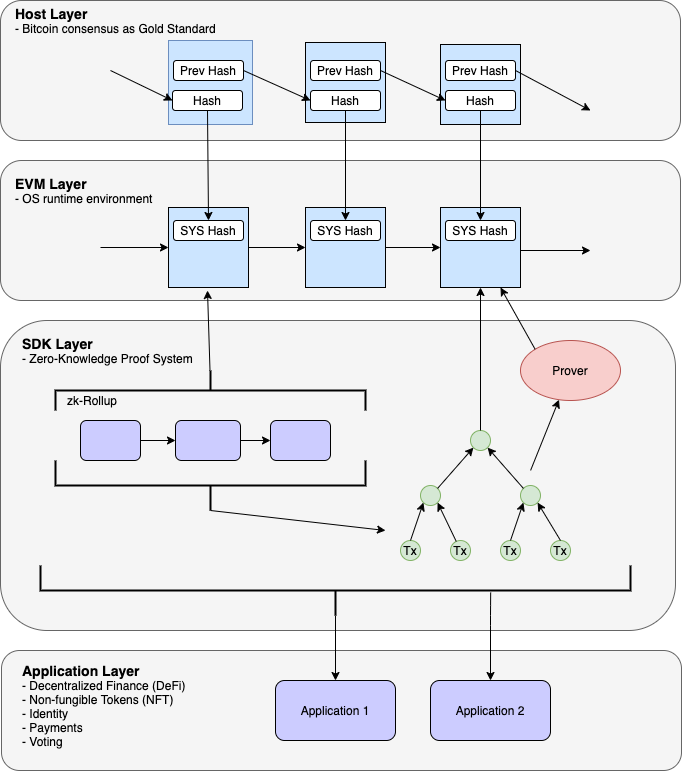
\includegraphics[width=3.5in]{img/4_layer.png}
\label{fig:tech_stack}
\caption{Proposed 4-layer tech stack for Syscoin} 
\end{figure} 

Surprisingly, these ideals represent a design that is not shared with any other project in the industry, including Bitcoin or Ethereum. We believe this design, fashioned together in a single protocol, could present a grand vision for a “World Computer” blockchain infrastructure.

Syscoin has already implemented Geth + Syscoin nodes in one application instance already (i.e., release 4.2). We foresee that there will not be any challenges associated with building a consensus basis working together to form a dual chain secured by Syscoin’s PoW.

\begin{figure}[h!]
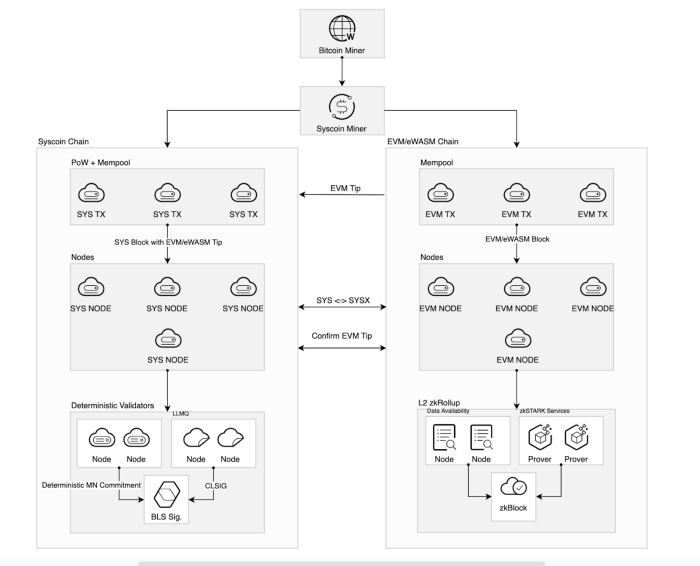
\includegraphics[width=3.4in]{img/fig_5.png}
\label{fig:proposed_design}
\caption{Proposed design} 
\end{figure} 

Figure 3 describes a system where nodes are running two sets of software processes, the Syscoin chain protocol and an EVM / eWASM chain protocol which are kept in sync through putting the EVM tip hash into the Syscoin block. Both have their own individual mempools and effectively the Ethereum contracts, tools and processes can directly integrate into the EVM chain. Note that the two chains are processes running on the same computer. Thus a SYS NODE and EVM NODE would be operating together on one machine instance (i.e., full node or masternode) with the ability to communicate with each other directly through Interprocess Communication (IPC). The intersection happens at three points:

\begin{enumerate}
\item Miner of the EVM chain collects the latest block hash and places it into the Syscoin block.
\item When validating Syscoin blocks nodes confirm the validity of the EVM tip by consulting the EVM chain software locally.
\item Fees for the EVM chain are to be paid in SYS. We will enable this through a similar working concept that we’ve already established (SysEthereum Bridge). We may also enable pre-compiles on the NEVM to extract Syscoin block hashes and Merkle roots to confirm validity of SYS to NEVM burn transactions.
\end{enumerate}

\begin{figure}[h!]
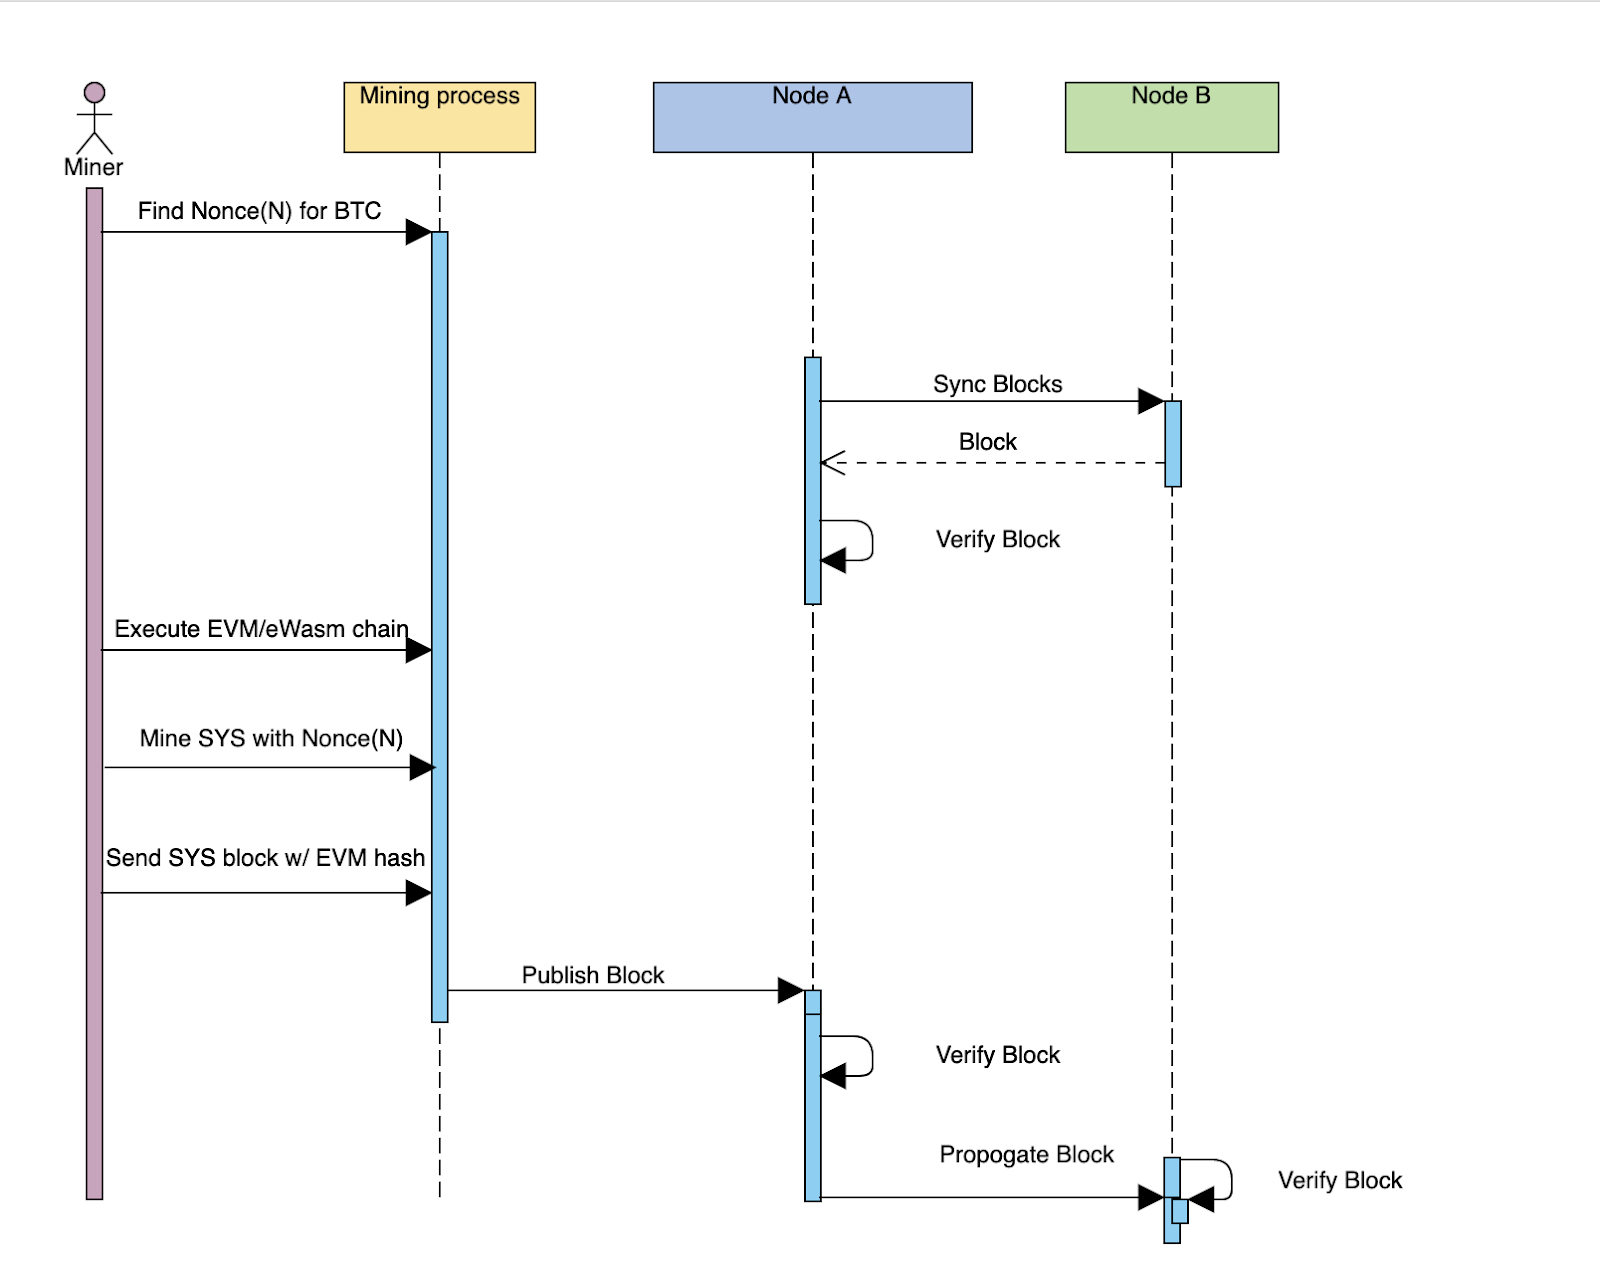
\includegraphics[width=3.4in]{img/fig_6.png}
\label{fig:tech_stack}
\caption{Merge mining on Syscoin} 
\end{figure} 

As seen in Figure 4, work done on BTC is reused to create SYS blocks through the merged-mining specification. Concurrently, the miner will execute smart contracts in the memory pool of the node running the EVM chain. Once a chain hash has been established post-execution, it will be put into a Syscoin block and published to the network. Upon receiving these blocks, every node would verify that the EVM chain, which can be locally executed (i.e., same as the miner), matches the state described by the Syscoin block. Technically, one would want to ensure both the latest and previous EVM block hashes inside of their respective Syscoin blocks are valid. The block $->$ evmblock $==$ evmblock \&\& block $->$ prev $==$ evmblock $->$ prev is all that is needed to link the chains together with work done by Bitcoin which is propagated to Syscoin through AUXPOW and can serve as a secure ledgering mechanism for the EVM chain.

Since (a) we may use eWASM; (b) there are paid full nodes running on the network; and (c) the mining costs are shared with Bitcoin miners, we should, therefore, be able to safely increase the amount of bandwidth available in the EVM chain while remaining secure from large uncle orphan rates. There has been much discussion as to what the safe block size should be on Ethereum. Gas limits are increasing as optimizations are made on the Ethereum network. However, since this network would be ledgered by the Syscoin chain through PoW, there should be no concern for uncle orphaning of blocks since the blocks must adhere to the policy set inside of the Syscoin block. We should therefore be able to increase bandwidth significantly and parameterize for a system that will scale globally yet still be centered around L2 rollup designs. In contrast to our design, Ethereum 2.0 centers around a Beacon chain and sharding served by a Casper consensus algorithm \cite{But17}. The needs of the Casper algorithm require a set of finality guarantees necessitating a move towards Proof-of-Stake (PoS). This has large security implications for which there may not be a formal analysis available for a long time \cite{Neu21}. Syscoin offers similar levels of scalability while retaining Nakamoto Consensus security. The simpler design that has been market tested and academically verified to work would result in a more efficient system as a whole with fewer unknown and undocumented attack vectors. Hence, we need only to consider researching the optimal parameterization of the gas limit taking into account an L2 centric system, as well as the safe number of users we expect to be able to serve before fee market mechanisms begin to regulate the barrier of entry for these users. This proposed system should be scalable enough to serve the needs of global generalized computation while sticking to the core fundamentals set forth in the design explained above.  Some theoretical scaling metrics will be included at the end of this article (our upcoming whitepaper will have more analysis on these numbers).

\subsubsection{Related Works}

The following organizations offer various open-source, third-party L2 scaling solutions:

\begin{itemize}
\item Starkware 
\item ZEXE(Aleo) 
\item Matter labs 
\item Hermez
\item Connext 
\end{itemize}

Starkware is built using a general-purpose language (Cairo) with Solidity (EVM) in mind \cite{Sta20b}, as is Matter labs with the (Zinc) language \cite{matter21}. Hermez developed custom circuits tailor-made to support fast transactions and Decentralized Exchange (DEX) capabilities \cite{hermez21}. These will be able to directly integrate into Syscoin without modification. As such, the optimizations and improvements they make should be directly portable to Syscoin, hence becoming partners to our ecosystem.

Aleo uses Zero knowledge EXEcution (Zexe) for zkSNARK proof creation through circuits created from R1CS constraints \cite{aleo21}. The interesting thing about Aleo is that there is a ledger itself that is purpose-built to only verify these Zexe proofs for privacy preserving transactability. The consensus is PoW, while the proof system involves optimizing over the ability to calculate the verifications of these proofs efficiently. The more efficient these miners become at verifying these proofs, the faster they are able to mine and thus the system provides sybil resistance by providing resources to verify Zexe proofs as a service in exchange for block creation. However, these proof creations can be done in parallel based on the business logic for the systems the developers need to create. There is no direct need for on-chain custom verification as these can be done in an EVM contract, similar to Cairo Generic Proving Service (GPS) verifier and Zinc Verification. The goal of Aleo is to incentivize miners to create specialized hardware to more efficiently mine blocks with verification proofs. However, provers can also do this as we have seen with Matter Labs’ recent release of FPGA to do more efficient zkSNARK proofs \cite{Glu20}. It is a desirable property to use PoW to achieve “world-view” consensus in Aleo; however they focus on private transactions. They are typically not batched and employ a recursive outer proof to guarantee execution of an inner proof where the outer proof is sent to the blockchain to be verified. This proof is a limited two-step recursion. Consequently, batching of arbitrary amounts of transactions is not supported. As a result, the cost of proof verification is relatively constant with a trade-off of limiting the recursion depth. Aleo is not meant to be a scalable aggregator of transactions, it is mainly oriented towards privacy in their zk-SNARK constructions using Zexe.

\subsubsection{Functional Overview}

For scalable simple payments, one can leverage our Syscoin Platform Token (SPT) asset infrastructure and payment channels to transact at scale. Unique characteristics of SPTs include a generalized 8 byte field for the asset ID which is split between the upper and lower 4 bytes; the upper 4 are issued and definable (ie., NFT use cases) and lower 4 are deterministic. This enables the ability to have a generalized asset model supporting both Non-fungible Tokens (NFT) and Fungible Tokens (FT) without much extra cost at the consensus layers. 1 extra byte is used for all tokens at best case and 5 extra bytes are used for NFT at worst case. See \cite{NFT21} for more information on Syscoin’s NFTs. This model promotes multiple assets to be used as input, and, consequently, as outputs, which suggests that atomic swaps between different assets are possible. This has some desirable implications when using payment channels for use cases such as paying in one currency when merchants receive another atomically. A multi-asset payment channel is a component that is desired so users are not constrained to single tokens within a network. Composability of assets, as well as across systems (such as user from one L2 to another), is a core fundamental to UX and a convenience that needs to be built into our next generation blockchain components, which we believe will enable mass adoption. The Connext box shows how potentially you can move from one L2 on one network to another as described in \cite{Bhu21}. This would promote seamless cross-chain L2 communication without the high gas fees. Since these L2s are operating under an EVM/eWASM model, there are many ways to enable this cross-communication.

An EVM layer will support general smart contracts compatible with existing Ethereum infrastructure and L2 rollups will enable massive scale. The different types of zkRollups will give businesses and rollup providers the ability to offer custom fee markets (i.e., pay for fees in tokens other than base layer token SYS). In addition, it will remove costs, and, thus, improve the scale of systems by offering custom data availability consensus modules. This design shares similarities to the zkPorter \cite{matter21} design where a smart contract would sign off on data availability checks that would get put into the ZKP as part of the validity of a zkBlock which goes on chain.

The overall idea of the zkPorter design is that the zkRollup system would be called a “shard”, and each shard would have a type either operating in “zkRollup” mode or operating in “normal” mode. This concludes that shards can define different consensus modules for data availability (censorship resistance mechanisms) via separating concerns around ledgering the world-view of the state (i.e., ZKP that is put on L1) and the data that represents the state. Doing so would allow shards to increase scale and offload costs of data availability to consensus participants.

A few note-worthy examples of consensus for data availability are:

\begin{enumerate}
\item Non-committee, non fraud proof based consensus for data availability checks. No $2/3$ online assumption; see \cite{But20}. 
\item Sublinear block validation of ZKP system. Use something like Lazy Ledger as a data availability proof engine and majority consensus; see ethresear.ch post \cite{Al20}. 
\item Use a combination of the above, as well as masternode quorum signatures for any of the available quorums to sign a message committing to data availability checks as well as data validity. Using masternodes can provide a deterministic set of nodes to validate decisions as a service. The data can be stored elsewhere accessible to the quorums as they reach consensus that it is indeed valid and available.
\end{enumerate}


\begin{figure}[h!]
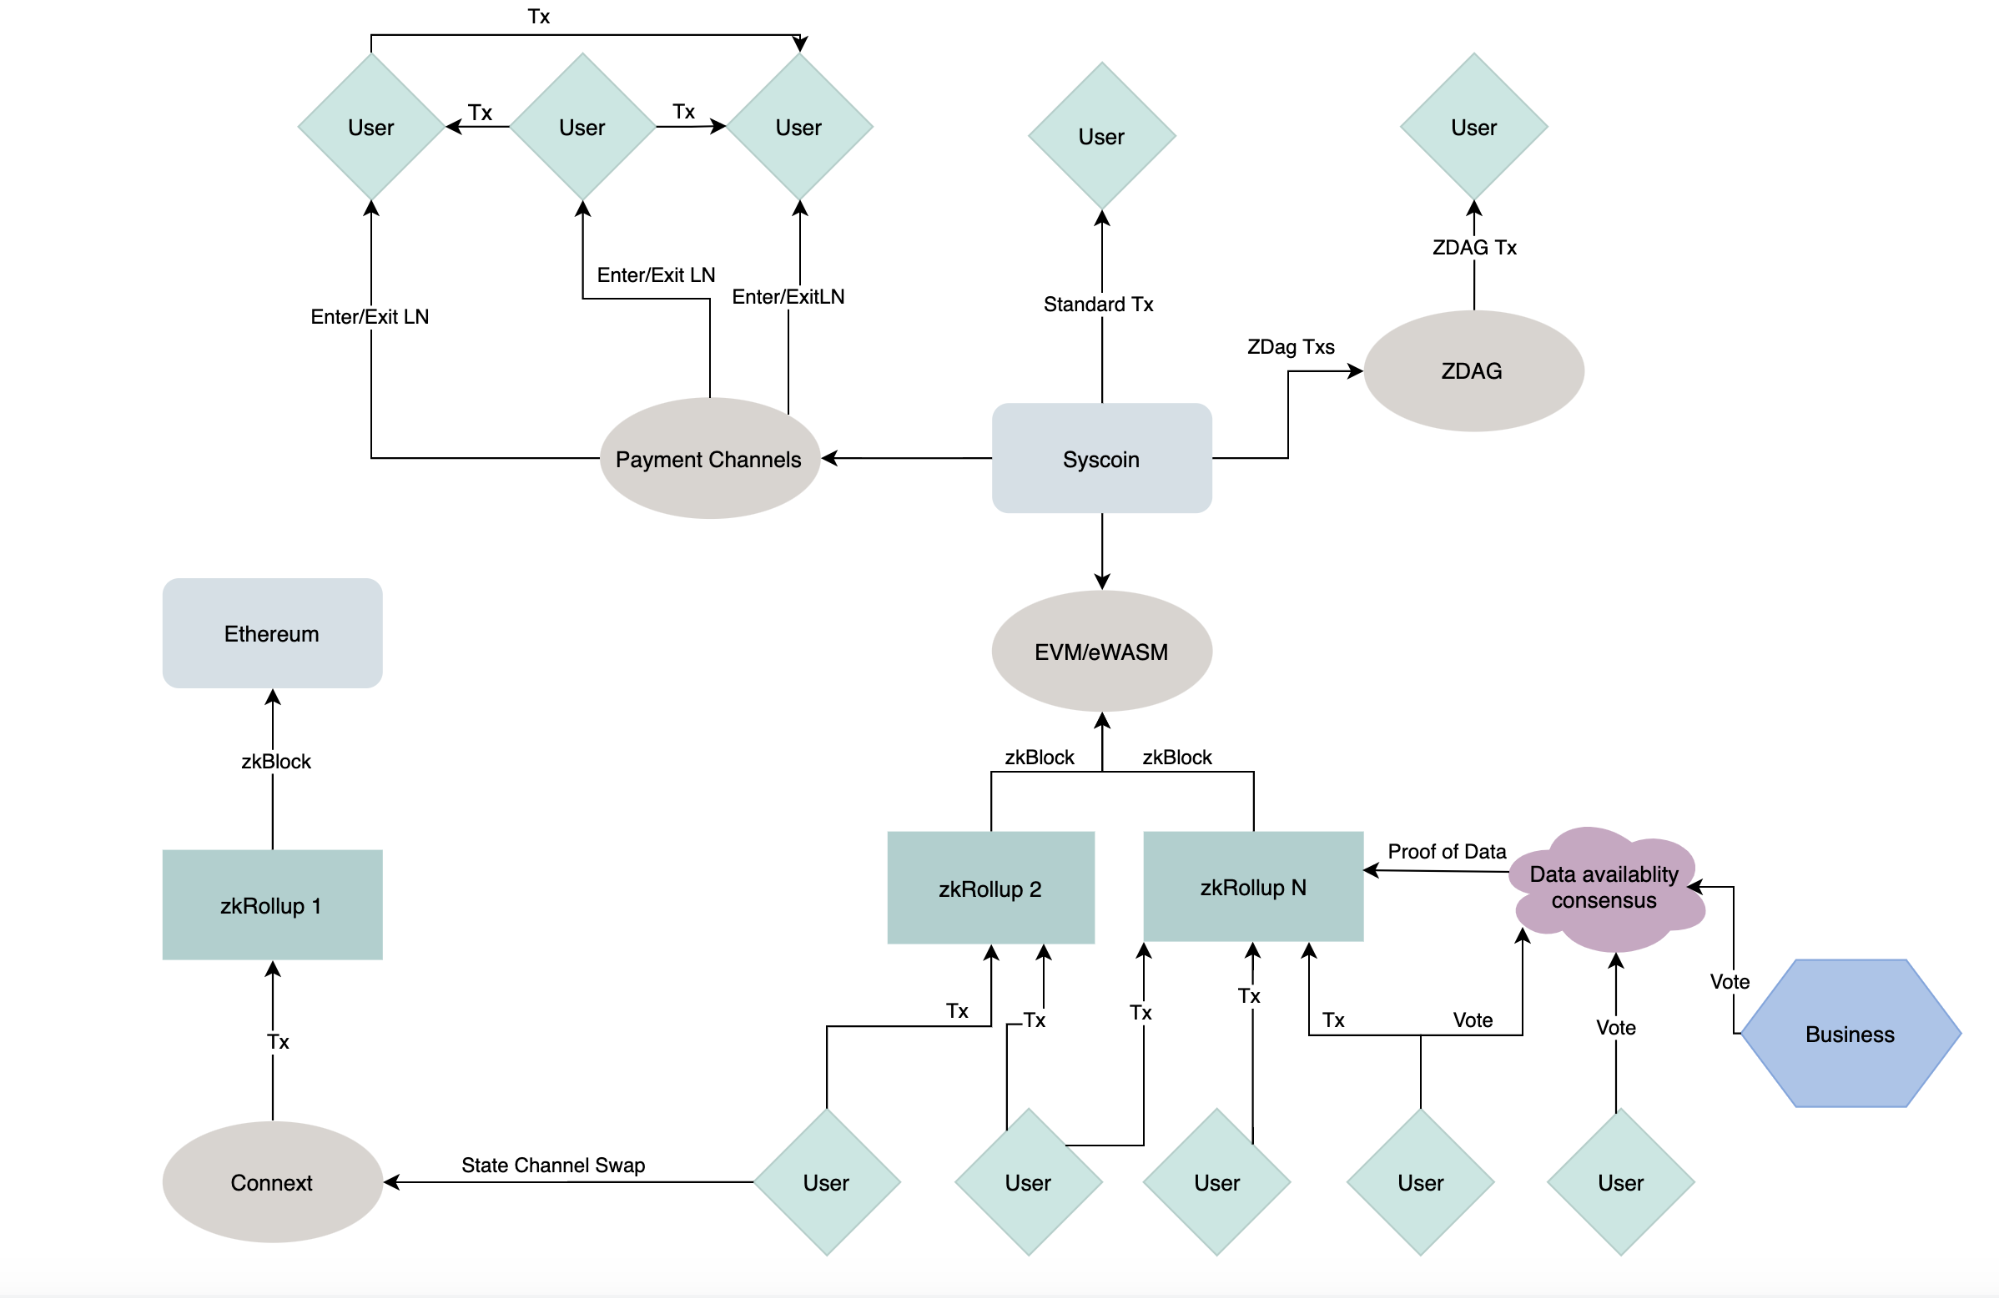
\includegraphics[width=3.4in]{img/nevm.png}
\label{fig:nevm}
\caption{Network EVM: High level description} 
\end{figure} 

\subsubsection{Optimistic vs ZkRollup}

ZKP are excellent for complex calculations above and beyond simple balance transfers. For payments, we feel UTXO payment channels combined with something like Z-DAG is an optimal solution. However, we are left with rollup solutions for generalized computation involving more complex calculations requiring consensus.

The solution we adopt has to be secured by L1 consensus that is considered decentralized and secure, which Syscoin has achieved via merged-mining with Bitcoin.

There are two types of rollup solutions today: (a) Optimistic rollups (OR); and (b) zkRollups; which offer trade-offs.

Consensus about which chain or network you are working on is a difficult problem that is solved for us by Nakamoto consensus. We build on that secure longest chain rule (supplemented by Chain Locks to prevent selfish mining) to give us the world-view of the rollup states. The executions themselves can be done once by a market of provers, never to be re-executed, only verified, suggesting it becomes an almost constant cost on an arbitrarily large number of executions batched together. Given these features, OR have the same capabilities with the exception of being editable without verifying executions. The role of determining the validity of that world-view is delegated to someone watching who provides guarantees through crypto-economics. ZKPs obviate crypto-economics on execution guarantees by use of cryptography.

Contrasting benefits between fraud proofs (optimistic) vs validity proofs (zk) can be found in \cite{Sta19}. The key takeaways from this article as to the superiority of validity proofs over fraud proofs include:

\begin{itemize}
\item Eliminate a nasty tail risk: theft of funds from OR via intricate yet viable attack vectors;
\item Reduce withdrawal times from 1–2 weeks to a few minutes;
\item Enable fast transaction confirmations and exits in practically unlimited volumes;
\item Introduce privacy by default.
\end{itemize}

An area often overlooked is interoperability. A generalized form of cross-chain bridging can be seen in Chain A locking tokens based on a preimage commitment by Chain B to create a zero-knowledge proof, followed by verification of that proof as the basis for manifesting equivalence on Chain B. Any blockchain with the functionality to verify these proofs could participate in the ecosystem.

In this article we take a zkRollup-centric world-view. However, we acknowledge that it can be replaced with other technologies should they be able to serve the same purpose. As an infrastructure we are not enforcing one or the other; as developers can build on what they feel best suits their needs. We believe we are close to achieving this, and that the technology is nearing the point of being ready for the vision set forth in this article.

\subsection{Evidence}

Since payment channels work with UTXOs and also benefit from on-chain scaling via Z-DAG, 16MB blocks (with segwit weight) assumed, we will see somewhere around 8MB-12MB effectively per minute (per block). We foresee that is sufficient to serve seven billion people who may enter and exit the payment channel networks once a year (ie, 2 transactions on chain per person per year) for a total of 14 Billion transactions. Let’s conservatively assume 8MB blocks and 300 bytes per transaction. Once on a payment channel, the number of transactions is not limited to on-chain bandwidth but to network related latencies and bandwidth costs. Therefore, we will conclude that our payment scalability will be able to serve billions of people doing 2 on-chain transactions per year, which is arguably realistic based on the way we envision payments to unfold; whether that is on a L2 or a payment channel network that will enable users to pay through instant transaction mechanisms. For on-chain, we have some metrics on Z-DAG throughput [1]; in the cases where someone needs to transact through point-of-sale using the Syscoin chain. The solution for payments ends up looking like a hybrid mechanism of on-chain (i.e., Z-DAG) and off-chain (i.e., payment channel) style payments.

Complex transactions such as smart contracts using zkRollups require a small amount of time to verify each proof. In this case, we assume that we will host data off-chain while using an off-chain consensus mechanism to ensure data availability for censorship resistance. Therefore, the only things that go on the chain are validity proofs. We will assume that we will assign 16MB blocks for the EVM chain per minute. 

In the Reddit bake-off estimates \cite{Sta20a}, Starkware showed that a proof size will be about 300kB for about 300k transactions batched together which will take about 60-80ms to verify and roughly 5 to 10 minutes to create such proofs. This was done using zk-STARKs, which present quantum resistance and no trusted setup.  Hence, zk-SNARKs offer smaller proofs and verification times at the expense of trusted setups and stronger cryptography assumptions (not post-quantum safe). We foresee that these numbers will improve over time as the cryptography improves, but current estimates suggest a rough theoretical capacity of around 1 Million offchain TPS. 

\subsubsection{Gas Costs and Block Sizing}

Starkware was able to process 300k transactions over 8 blocks with a total cost of 94.5M gas; final throughput was 3000 TPS (see Reddit bake-off estimates \cite{Sta20b}). For the following calculations, let’s assume one batch-run to be 300k transactions. Ethereum can process $\sim$ 200kB of data per minute, with a cost limit of 50M gas per minute. Therefore, considering the Starkware benchmark test, and assuming a block interval of 13 seconds, we would achieve ~ 3000 TPS (ie,  300 k transactions per batch-run / (8 blocks per batch-run * 13 seconds per block))

It is estimated that Syscoin will be able to process $\sim$ 16MB of data per minute on the EVM layer (ie, NEVM in Fig 3), which is $\sim$ 80x gain over Ethereum; thus a cost limit of 4B gas (ie, 80*50M) per minute. Therefore, if the Starkware benchmark test was run on Syscoin, it is estimated that Syscoin could run the equivalent of 42 batch-runs per minute (i.e., 4B gas per minute / 94.5M gas per batch-run). That would result in an equivalent of 210k TPS (i.e., 42 batch-runs per minute * 300k transactions per batch-run / 60 seconds per minute).

If we were to consider using Validum on the Syscoin EVM layer we estimate that we could achieve 800 batch-runs per minute (i.e., 4B gas per minute / 5M gas per batch-run). That would equate to an equivalent of 4M TPS (i.e., 800 batch-runs per minute * 300k transactions per batch-run / 60 seconds per minute).

\begin{figure}[h!]
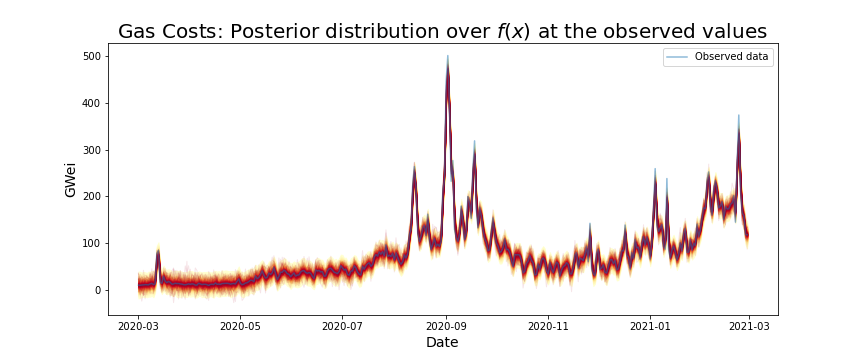
\includegraphics[width=3.7in]{img/eth_gas_costs.png}
\caption{Ethereum gas gosts in Gwei from Mar 2020 to Mar 2021. The region about the observed gas costs represents the posterior distribution of $f(x*)$ given observations, $y$, for a set of dates, $x*$; see Appendix G for details}  
\label{fig:eth_gas_costs}
\end{figure} 

\begin{figure}[h!]
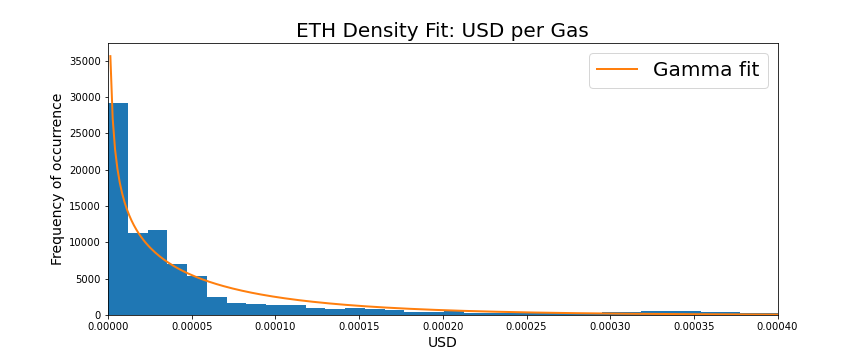
\includegraphics[width=3.7in]{img/eth_usd_density.png}
\caption{Gamma fit of Ethereum gas costs in USD using generated samples from Figure \ref{fig:eth_gas_costs} and corresponding ETHUSD prices} 
\label{fig:eth_usd_density}
\end{figure} 

The results from these aforementioned estimates have been tabulated in Table \ref{table:gas_cost_estimates}; more specifically, median estimates (along with its 5th and 95th percentiles) for the costs in USD terms for both ETH and NEVM. The estimates for Ethereum were determined using historical gas costs from March 2020 to March 2021 as shown in Figure \ref{fig:eth_gas_costs}, and its distribution fit in Figure \ref{fig:eth_usd_density}.

\begin{figure}[h!]
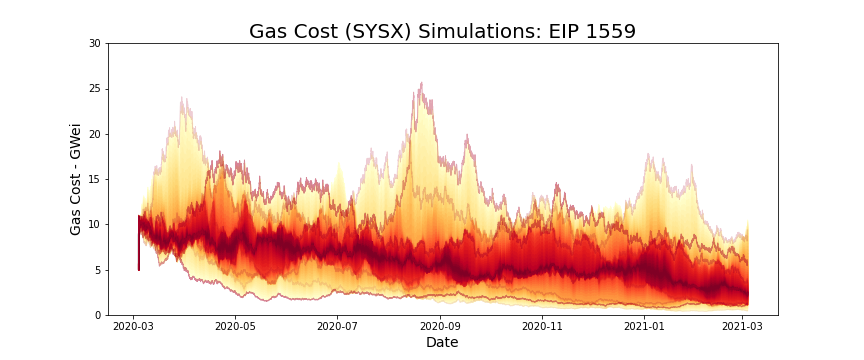
\includegraphics[width=3.7in]{img/sysx_gas_costs_eip_1559.png}
\caption{Gas cost simulations of NEVM using EIP-1559; see Appendix G. This graph shows the non-stationary decline in price over time. To our knowledge, treating this non-stationary behaviour requires better understanding of the mathematical assumptions, which have not yet been analytically researched.} 
\label{fig:sysx_gas_costs_eip_1559}
\end{figure} 

\begin{figure}[h!]
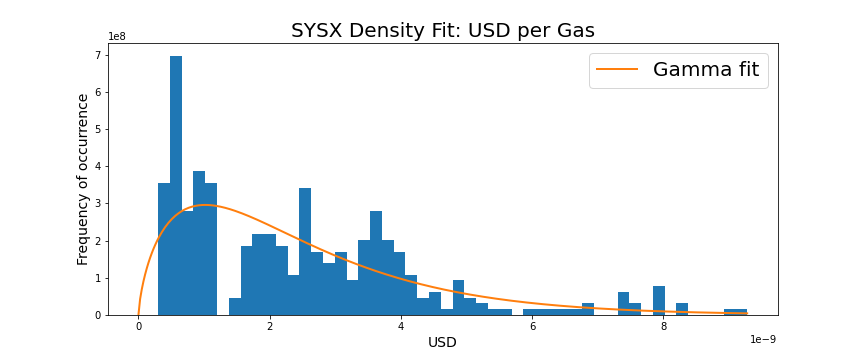
\includegraphics[width=3.7in]{img/sysx_usd_density.png}
\caption{Gamma fit of NEVM gas cost simulations in USD using generated samples from Figure \ref{fig:sysx_gas_costs_eip_1559} and SYSUSD prices from Mar 2020 to Mar 2021. These estimates are hypothetical, and will be subject to market price of SYS. Note that if significant adoption occurs due to future demand for cost effective alternatives we foresee future prices being slightly higher.} 
\label{fig:sysx_usd_density}
\end{figure} 

With regards to the NEVM cost estimates, simulated gas costs were generated using Ethereum's proposed EIP-1559 (Figure \ref{fig:sysx_gas_costs_eip_1559}) and an alternative pricing mechanism that Syscoin is currently exploring. This alternative approach is called the BLock Occupancy Cost (BLOC) function (\ref{fig:bloc}), and is driven by the occupancy of the previously generated block; see Appendix D for details.

\begin{table*}[h!]
\centering
\begin{tabular}{ |c|c|c|c|c|c|c|c|c|c|   } 
\hline
Chain & Gas  Limit & Block Time & Mode & Cost  & Amortized  & Total TPS & \multicolumn{3}{|c|}{USD / 300K Tx (Mar 20 to Mar 21) } \\
 &  &  &  &  300K Tx  & Cost per Tx  &  & median & lwr 5\% &  upr 95 \% \\ 
\hline
\multirow{3}{*}{ETH} & \multirow{3}{*}{12.5M} & \multirow{3}{*}{13 sec} & L1 & 6.3B gas  & 21,000 gas  & ~45 & 159,328.24 & 10,669.40  & 1,914,394.79  \\ 
\multirow{3}{*}{} & \multirow{3}{*}{} & \multirow{3}{*}{} & L2 zk-Rollup & 94.47M gas  & 315 gas & ~3,000* & 2,389.16 & 159.99  & 28,706.81 \\ 
\multirow{3}{*}{} & \multirow{3}{*}{} & \multirow{3}{*}{} & L2 Validium  & 5M gas  & 17 gas & ~56,000** & 126.45 & 8.47  & 1,519.36 \\ 
\hline

\multirow{3}{*}{NEVM} & \multirow{3}{*}{10B} & \multirow{3}{*}{150 sec} & L1 & 6.3B gas  & 21,000 gas  & ~3,100*& 1.92496 & 0.97008 & 4.51653 \\ 
\multirow{3}{*}{} & \multirow{3}{*}{} & \multirow{3}{*}{} & L2 zk-Rollup & 94.47M gas  & 315 gas & ~210,000** & 0.02887 & 0.01455 & 0.06773 \\ 
\multirow{3}{*}{} & \multirow{3}{*}{} & \multirow{3}{*}{} & L2 Validium  & 5M gas  & 17 gas & ~4,000,000 & 0.00153 & 0.00077  & 0.00358 \\ 
\hline

\end{tabular}
\caption{Comparison of Gas and USD costs between ETH and NEVM. The confidence intervals for USD estimates were determined using historical gas costs for ETH (see Figure \ref{fig:eth_gas_costs}), and simulated gas costs for NEVM (see Figure \ref{fig:sysx_gas_costs_eip_1559}) using EIP-1559.}
\label{table:gas_cost_estimates}
\end{table*}

Because of the higher throughput capabilities of baseline EVM, we may look to dynamically adjust costs of the gas limits \cite{Che17} to thwart DOS attacks.

So far we have looked at EIP-1559 and the BLOC model, which both dynamically adjust gas costs. A third option we are looking at is to maintain the auctioning with a dynamic blocksize system. To facilitate this we developed a methodology driven by block failure frequency, see Appendix \ref{appendix:block_resize} for the details. 

\subsubsection{Discussion}

The aforementioned calculations support the full State Safety of the main chain secured by Bitcoin, and no asynchronous network assumptions, which make theoretical calculations impractical in many other claims of blockchain throughput due to execution model bottlenecks. These results were extrapolated based on real results with constant overhead added that becomes negligible with optimizations. It is important to  note that transactions in this strategy are not re-executable; there is little to no complexity in this model other than verifying succinct proofs. The proof creation strategy is parallelized organically using this model. The verifications on the main chain can also be parallelized as they are executed on separate shards or rollup networks. Dual parallel execution and verification gives exponentially more scalability than other architectures. Additionally, depending on the business model, privacy can be built into these models at little to no extra cost. Lastly, we suggest  these are sustainable throughput calculations and not burst capacity numbers, which would be much higher (albeit with a marginally higher fee based on fee markets). For example, Ethereum is operating at 15 TPS, but there are around 150k transactions pending, and the average cost is about 200 Gwei currently. The fee rate is based on the calculation that it  takes around 10k seconds to clear, assuming this many transactions, no new transactions, and there is demand to settle earlier. Extrapolating on 4M TPS the ratio would become 40B transactions pending with 4M TPS to achieve the same fee rate on Ethereum today assuming the memory pool is big enough on nodes to support that many pending transactions. Since masternodes on Syscoin are paid to provide uptime, we can expect network bandwidth to scale up naturally to support higher throughput as demand for transaction settlement increases. Today, the ability to transact at a much higher rate using the same hardware provides greater scalability than the state-of-the-art in blockchain design without the added desired caveat of avoiding asynchronous network assumptions. We believe the proposed design will become the new state-of-the-art blockchain, which is made viable due to its security, flexibility and parallelizable computational capacity.

With regards to uncle rates with higher block sizes, we speculate that the NEVM will make uncle rates negligible through the use of the PoW chain mining Syscoin along with Chain Locks. We provide intuition that block sizes can be increased substantially without affecting network health. Furthermore, gas limits can be adjusted by miners up to 0.1\% from the previous block and so a natural equilibrium can form where even if more than 4B gas is required it can be established based on demand and how well the network behaves with such increases. 

\subsubsection{Decentralized Cost Model}

Decentralized cost models lead to efficiency gains in economies of scale. We set forth a more efficient design pertaining to user intent. This design uses the UTXO model to reflect simple state transitions and a ZKP system for complex computations leading to state transitions. This leads to ideal scalability for a system by allowing people to actively make their trade-off within the same ecosystem, driven by the same miners securing that ecosystem backed by Bitcoin itself.

Furthermore, a decentralized cost model contributes to scalability in that ZKP gates can generalize complex computation better than fee-market resources like gas or the CPU/memory markets of EOS, etc. This leads to more deterministic and efficient consumption of resources maximizing efficiency in calculations. It also provides an opportunity for those to scale up or down based on economic incentives without creating monopolistic opportunities unlike ASIC mining. In other words, the cost is dictated by what the market can offer, via the cost of compute power (as dictated by Moore's law) instead of constrained costs of doing business on the blockchain itself. This model could let the computing market dictate the price for gas instead of being managed by miners of the blockchain. The miners would essentially only dictate the costs of the verification of these proofs when they enter the chain rather than the executions themselves.

We can begin to see computational optimization through hardware happening with ZKP, and with a decentralized cost model it will be much simpler to understand costs of running prover services, as well as know how the costs scale based on the number of users and parameters of systems that businesses may employ. All things considered, it will be more efficient to make accurate decisions on data availability policies and the consensus systems needed to keep the system censorship resistant and secure.

Rollups will be friends. That is, users of one rollup system doing X TPS and users of another doing Y TPS, with the same trust model, will in effect get us to global rates of X*Y (where X is TPS of the sidechains/rollups and Y is the number of sidechains and rollups that exist). X is fairly static in that the execution models of rollups do not change drastically (and if they do, the majority of those rollup or sidechain designs end up switching to the most efficient design for execution over time).

\subsection{Tokenomics}

A good monetary system must exhibit some form of year over year inflation in supply, which is well understood by economists. With this project, there are both inflationary and deflationary pressures pushing on the supply. Hence, it is important to ensure that the inflationary pressure coming from the block rewards outpaces the deflationary pressure coming from the fee burning. 

The current rewards for Syscoin 3 are 38.5 per block deflated 5\% per year with allocations of 67.5\% to masternodes, 22.5\% to miners and 10\% to governance proposals. When the transition to the NEVM occurs, the fee structure will change to EIP-1559 which includes: (a) an additional minting of 100M additional supply; (b) fee burning with an indeterminate block size; and (c) an elimination of max supply cap on SYS.

To understand the inflationary side, here is the setup under this new protocol starting Jan 2022 which is slated generate 86.8 SYS per block which occurs every 2.5 minutes. This breaks down to 58.62 SYS per block for masternodes, 19.52 SYS per block for Miners, and 8.675 SYS per block for Governance. These masternode rewards get bumped to 79.15 SYS for 1 year seniority and 117.25 SYS for 2.5 year seniority. As with Syscoin 3, the above figures will deflate 5\% per year. Once miner rewards and governance payouts reach near zero on the Syscoin mainchain, masternode holders will continue to receive SYS at a minimum of 5.275 SYS and a maximum of 10.55 SYS for full seniority nodes. An additional 0.25\% will be rewarded on the NEVM chain which will equate to 10.55 SYS per block, and will not change year over year.

Next, to understand the deflationary side we modelled the historical transaction fee data from Ethereum as shown in Fig. \ref{fig:tx_burn}, and applied that model to our tokenomics model. For methodology, please refer to Appendix \ref{appendix:tx_fee_burn}.

\begin{figure}[h!]
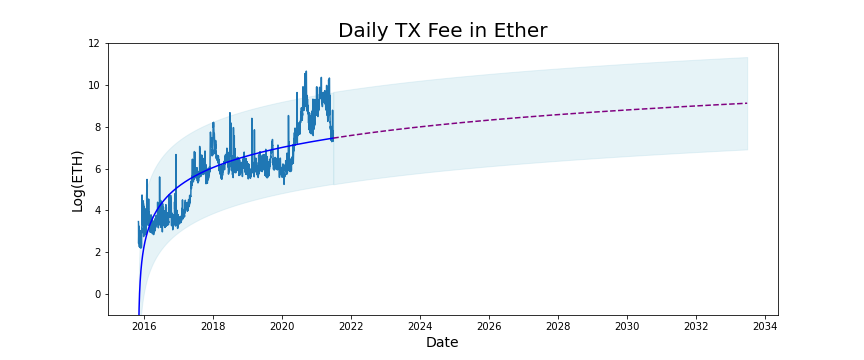
\includegraphics[width=3.7in]{img/eth_daily_tx_fee.png}
\caption{Ethereum daily transaction fee burn with projections.} 
\label{fig:tx_burn}
\end{figure} 

Finally, for our supply model we combine the two components by taking the block rewards and subtracting off what is presumed to be burned through transaction fees as shown in Fig. \ref{fig:tx_delay}. For the lower bound we assume all masternodes to have less than one year seniority, and for the upper bound   we assume all masternodes to have full senority.

\begin{figure}[h!]
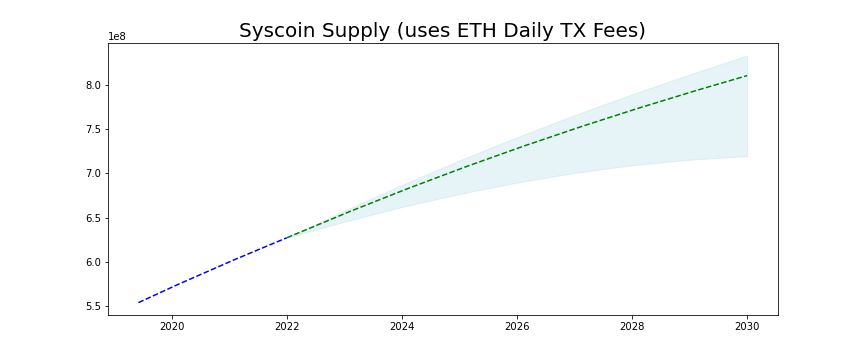
\includegraphics[width=3.7in]{img/syscoin_daily_supply.png}
\caption{Projected daily supply (Dec 6$^{th}$ start date) is comprised of two main components: (a) block rewards; and (b) fee burning. As long as the lower bound of the projected block reward growth outpaces the burn rate shown in Fig. \ref{fig:tx_burn} then supply is inflationary.} 
\label{fig:tx_delay}
\end{figure} 


\begin{table}[h!]
\centering
\begin{tabular}{ |c|c|c|c| } 
\hline
 & \multicolumn{3}{|c|}{ Supply } \\
 Date (1$^{st}$ of Jan) & Pred & Lwr & Upr \\
\hline
2022 & 727,569,000 & 726,910,000 & 727,822,000 \\
2023 & 753,371,000 & 744,032,000 & 756,867,000 \\
2024 & 777,884,000 & 759,626,000 & 784,452,000 \\
2025 & 801,235,000  & 773,518,000 & 810,716,000 \\
2026 & 823,358,000  & 785,487,000 & 835,584,000 \\
2027 & 844,374,000 & 795,454,000 & 859,192,000 \\
2028 & 864,340,000 & 803,267,000 & 881,560,000 \\
2029 & 883,359,000 & 808,811,000 & 902,924,000 \\
2030 & 918,496,000 & 812,038,000 & 923,102,000 \\
2031 & 934,758,000 & 812,891,000 & 942,240,000 \\
2032 & 950,250,000 & 811,302,000 & 960,400,000 \\
\hline
\end{tabular}
\caption{Supply prediction using new NEVM protocol beginning Jan 2022 through to Jan 2032 with lower and upper thresholds}
\label{table:pow_vs_pos}
\end{table}

\subsection{Applications}

Commercial enterprises may start to create proprietary prover technologies where costs will be lower than market in an attempt to create an advantage for user adoption. This design is made possible since the code for the prover is not required for the verifier to ensure that executions are correct. The proof is succinct whether or not the code to make the proof is available.

While the barrier to entry is low in this industry, we have seen the open-source model and its communities optimize hardware and software and undergo academic peer review using strategies  that outpace private funded corporations. It is plausible that this will continue to play out over the long term. However, an organic market will likely form on its own, forging its own path leading to mass adoption through capitalist forces. The point here is that the privately funded vs. open source nature of proving services does not change the mechanism of secure and scalable executions of calculations that are eventually rooted to decentralized and open ledgers secured by Bitcoin.

The utmost interesting propositions are the verticals that become possible by allowing infrastructure that is parameterized to scale into those economies where they are needed most, and where trust, security and auditability of value are concerns. Smart cities, IoT, AI and digital sovereignty are large markets that intersect with blockchain as a security blanket. Although ZKPs are tremendously useful on their own, applying them to consensus systems for smart contract executions drive them to another level due to the autonomous nature of “code-is-law” and provable deterministic state of logic. We believe a large part of the future economy will depend on many of the ideas presented here. Blockchain Foundry is working with commercial and enterprise adopters of blockchain technology. Our direct interaction with clients combined with our many collective years of experience in this field are reflected in this design.


\section{Specifications}
\label{section:specs}

General specifications for Syscoin 4.3:

\begin{description}[font=$\bullet$~\normalfont\scshape\color{blue!50!black}]
\item \textbf{Block time:} 150 seconds
\item \textbf{Halving interval:} 210240 (1 year)
\item \textbf{Base Rewards:}  96.25 SYS per block deflated 5 percent every 210240 blocks
\item \textbf{NEVM Rewards:}  10.55 SYS per block (not deflated). EIP1559 model
\item \textbf{Governance Proposals:}  10 percent of Base Rewards paid out every 17520 blocks (1 month)
\item \textbf{Miner/Masternode Subsidy:}  90 percent of Base Rewards. 25 percent of this value goes to miner, 75 percent of this value goes to masternode
\item \textbf{Masternode Minimum Subsidy:} 5.275 SYS (can not go below this amount even accounting for deflation)
\item \textbf{Fees:}  50/50 split between miner and masternode
\item \textbf{Consensus:} PoW is SHA256. Merge-mined with Bitcoin
\item \textbf{Masternode collateral requirement:} 100,000 SYS
\item \textbf{Masternode seniority}: 35 percent increase after 210240 blocks (1 year), 100 percent increase after 525600 blocks (2.5 years)
\end{description}


\section{Summary}
\label{section:summary}
We have presented what is currently under way for Syscoin 4, which will come in the form of a four-layer tech stack to work with the Ethereum ecosystem via our NEVM. With the ever-increasing cost of gas prices, we present the data showing a 1000x+ improvement over Ethereum 2.0 in efficiency in terms of low gas cost per transaction. Syscoin will utilize the best features of the top two cryptocurrencies, namely Bitcoin and Ethereum. Hence, Syscoin will provide the security offered by Bitcoin while maintaining the programmability of Ethereum. Scalable applications will be mounted on this system via ZKPs which will introduce our proposed decentralized cost model on Ethereum gas fees.

\appendices

\section{Security: PoW vs. PoS}

Proof of Stake (PoS) systems have security threats that are not inherent in Proof of Work (PoW) systems as outlined in Table \ref{table:pow_vs_pos}, of which Bitcoin employs. Hence, PoS is less secure than PoW. In terms of security, we call the Bitcoin PoW protocol the gold standard, which is the same security mechanisim that Syscoin uses. 

\begin{table}[h!]
\centering
\begin{tabular}{ |c|c|c|c| } 
\hline
 & \multicolumn{3}{|c|}{ Vulnerability } \\
 Attack type & PoW & PoS & Delegated PoS \\
\hline
Short range attack & - & + & - \\
Long range attack & - & + & + \\
Coin age accumulation attack & - & maybe & - \\
Precomputing attack & - & + & - \\
Denial of service & + & + & + \\
Sybil attack & + & + & + \\
Selfish mining & - (chainlocks) & - & - \\
\hline
\end{tabular}
\caption{Comparing PoW to PoS consensus mechanism; plus sign (+) indicates vulnerability; see \cite{Bit15}. As shown, PoW system has the least number of vulnerabilities}
\label{table:pow_vs_pos}
\end{table}

\section{ZDAG Fundamentals}

Zero-Confirmation Directed Acyclic Graph (Z-DAG) is an instant settlement protocol that solves the 'fast-transaction' problem. It functions by using a Directed Acyclic Graph (DAG) where validating nodes verify the sequential ordering of transactions that are received in their memory pools. More specifically, Syscoin approach is centred around the verification of signatures and relaying of transactions. It does this by prioritizing the relay of transactions over signature verification and recipient receives funds faster; see Figure \ref{fig:dag_tx}. See Appendix A in \cite{Sidb18} for the verification process.

\begin{figure}[h!]
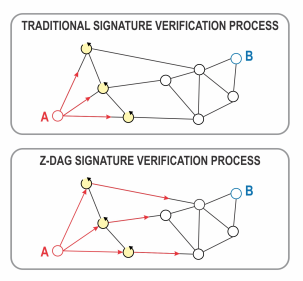
\includegraphics[width=3in]{img/dag_tx.png}
\caption{Traditional blockchain networks require each node to first check the signatures of incoming transactions before relaying them; this blocking technique bottlenecks broadcasting speed. The Z-DAG process as displayed above immediately relays transactions before checking signatures, resulting in significantly faster movement across the network} 
\label{fig:dag_tx}
\end{figure} 


\subsection{Transmission Path}

The expected number of common peers between k masternodes is:

\begin{equation}
E\{cp_{k}\} = pk -m \left(1 - \left(1 - \frac{p}{m}\right)^{k}\right),
\end{equation}
where $p$ is the number of common peers, and $X_{i}$ is 1 when the $i^{th}$ masternode is a common peer and 0 otherwise. The probability of having $n$ common peers is given by: 

\begin{equation}
P(|cp| = n) = \frac{\binom{M}{c} \binom{M-c}{p-c} \binom{M-p}{p-c} }{\binom{M}{p}}
\end{equation}

\subsection{Transmission Delay}

Using a dataset (containing 2086 samples) of average transmission times of ten transmissions between two hosts, it was modelled using the Gamma distribution as shown in Figure \ref{fig:tx_delay}. Using this model, the probability of transmission arriving in a given time can be estimated at various time points.

\begin{figure}[h!]
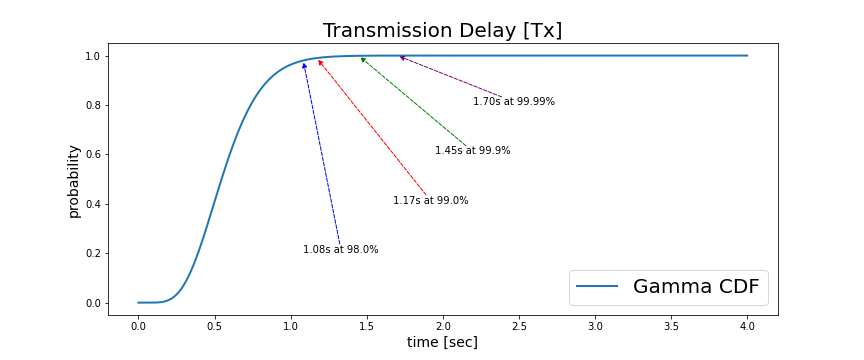
\includegraphics[width=3.7in]{img/transmission_delay.png}
\caption{Probability of Tx arrival after $5$ hops modelled via $X \sim Gamma(7.358,0.0777)$} 
\label{fig:tx_delay}
\end{figure} 

\section{Zero Knowledge Proofs Fundamentals}

The motivation of a Zero Knowledge Proof (ZKP) is to allow for one party (ie, prover) to convince another party (ie, verifier) of facts without revealing information (ie, zero knowledge). An example of a ZKP would be: allowing a subscriber (ie, prover) to gain access to an online service (ie, verifier) without revealing any personal data, other than the fact than that party is a paid subscriber. A ZKP must satisfy three conditions:

\begin{enumerate}
\item \textbf{Completeness:} If statement is true, verifier will be convinced by prover
\item\textbf{Soundness:} If statement is false, a cheating prover cannot (except with some small probability) convince verifier it is true
\item \textbf{Zero-knowledge:} If statement is true, verifier knows nothing else
\end{enumerate}

\begin{figure}[h!]
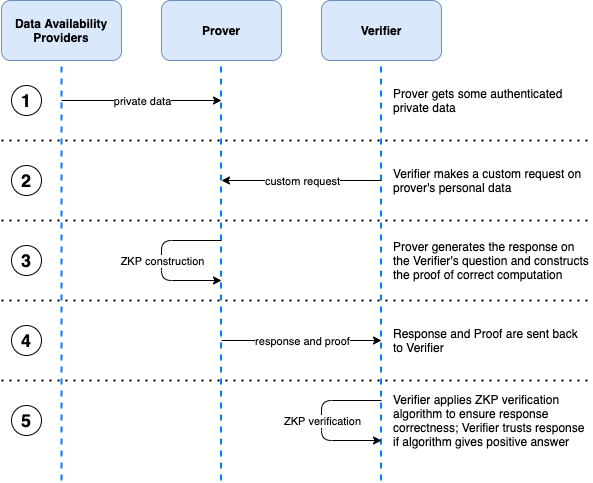
\includegraphics[width=3.7in]{img/zkp.png}
\caption{Data exchange in a Zero-knowledge proof system} 
\label{fig:zkp}
\end{figure} 

There are two types of ZKP:

\begin{enumerate}
\item \textbf{Interactive ZKP:} Comprised of multiple challenge / response messages (commitment, challenge and response); requires a stable communication channel
\item \textbf{Non-interactive ZKP:} Only needs single message and is more efficient; can be run offline
\end{enumerate}
zk-SNARK and zk-STARKS are types of Non-interactive ZKP , where no interaction is required between prover and verifier.

\section{Block Occupancy Cost (BLOC) Function}

We considered two approaches to model the gas costs, $y_{c,k}$ at the $k^{th}$ block, using model 1:
\begin{equation}
\mathbf{y}_{c,k} = \dfrac{1}{\gamma}\log\left(\dfrac{1+\mathbf{x}_{o,k-1}}{1-\mathbf{x}_{o,k-1}}\right) + \mathbf{y}_{c,0};
\end{equation}
and model 2:
\begin{equation}
\mathbf{y}_{c,k} = \left| \dfrac{1}{\gamma(\mathbf{x}_{o,k-1}-1)} \right| + y_{c,0} - \dfrac{1}{\gamma},
\end{equation}
where $x_{o,k} \in [0,1] \forall k$ is the block occupancy, $y_{c,0}$ is the base cost, and $\gamma$ is an adjustable scaling term. We call $y_{c}$ the BLock Occupancy Cost (BLOC) function; see Figure \ref{fig:bloc}.

\begin{figure}[h!]
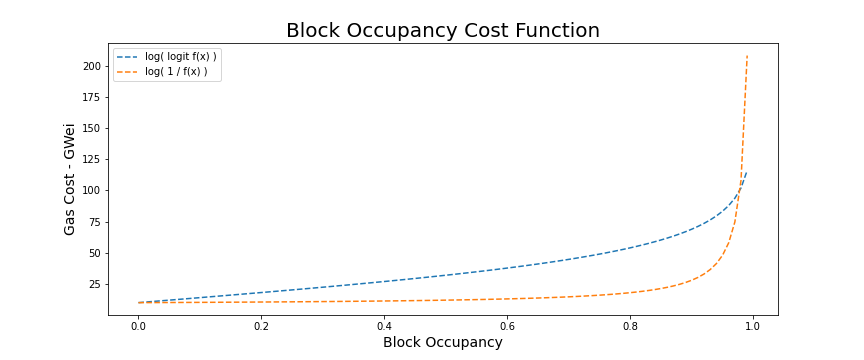
\includegraphics[width=3in]{img/blk_occupancy_cost_fn.png}
\caption{BLock Occupancy Cost (BLOC) functions; model 1 and 2} 
\label{fig:bloc}
\end{figure} 

Other variants of \textbf{y}$_{c}$ can be utilized highlighting various characteristics. For instance, Model 1 has the characteristic of being less volatile, but with a higher expected base cost than Model 2.

\section{Block Occupancy and Gas Simulations}

To simulate arbitrary block occupancies, we use the Beta distribution:

 \begin{equation}
\mathbf{x}_{o,t} \sim Beta(\alpha_{t},\beta_{t})
 \end{equation}
 where $t$ is time, and $\beta_{t} = 1-\alpha_{t}$
 
To exhibit slow upward growth over time for $\alpha_{t}$, we used a MinMax scaled ARIMA(0,1,1) model, otherwise known as a simple exponential smoothing model with growth, which is of the form:

\begin{equation}
\hat{\alpha'}_{t} = \mu + \alpha'_{t-1} - \theta_{1}\epsilon_{t},
\end{equation}
and then applied MinMax scaling to ensure $\alpha_{t} \in [0,1]$:
\begin{equation}
\hat{\alpha_{t}} = \dfrac{\alpha'_{t} - min(\alpha'_{t})}{  max(\alpha'_{t}) - min(\alpha'_{t}) }.
\end{equation}

Block Occupancy simulations, \textbf{x}$_{o,t}$, were fed into the BLOC function, to achieve a set of gas simulations, \textbf{y}$_{c,t}$, at each instance of time $t$.

\section{Block Resize on Failure Model}
\label{appendix:block_resize}

This Block Resize on Failure model dynamically adjusts the blocksize based on time to last block failure. If the time interval between failures is short then the probability of failure is high and the size for the next block gets decreased. However, when the time interval between failures is long then the probability of failure is low and the size for the next block size gets increased. This methodology is updated upon each failure, and consists of three main steps which include:
\begin{itemize}
\item Generate a Kaplan Meier estimator based on last N failures
\item Using time interval between last failure get estimated probability of failure using Kaplan Meier estimator
\item Feed the estimated probability of failure into a block size transfer function to get the block size adjustment for the next block
\end{itemize}

The goal of the Kaplan Meier estimator is to estimate the survival function, $S$, defined as:
\begin{equation}
S(t) = Pr(\tau > t),
\end{equation}
where $t$ is time, and  $\tau > 0$ be a random variable. The survivor function for the Kaplan Meier estimator function is given by:
\begin{equation}
\hat{S}(t) = \prod_{i; t_{i} < t} 1- \frac{d_{i}}{n_{i}}
\end{equation}
where $t_{i}$ is a time when at least one black failure happened, $d_{i}$ the number of failures, and $n_{i}$ the blocks that have not failed. 

The block size transfer function constructed from the following logit function:
\begin{equation}
y_{tr} = -2*A*\frac{e^{k(x-x_{0})}}{1+e^{k(x-x_{0})}} + A
\end{equation}
where preconfigured parameters ${A,k}$  determine how aggressive the resizing is upon each block failure. These parameters are typically determined aprior based on simulations run on the test net. 

\section{EIP-1559}

EIP-1559 is a new proposed pricing mechanism for the Ethereum protocol that includes a stationary network fee during states of no congestion which dynamically adjusts during states of congestion. The original gas fee model uses a auction system where miners choose transactions with the highest bids. This has led to several inefficiencies such as instability of blockchains with no reward, needless delays, fee overpayment, and mismatch fee levels between volatility ad social cost.

The basic premise of the new proposal begins with setting the base fee which increases when the network capacity exceeds the target per-block gas usage, and decreases when the capacity is below the target. The calculation of the updated basefee, $b_{k+1}$ at the $k+1^{th}$ block,  is as follows:

\begin{eqnarray} \label{eq:eip1559}
b_{k+1} = b_{k} f_{k}, \\
f_{k} = 1 + \dfrac{\delta_{k}}{c}
\end{eqnarray}
where $\delta_{k} = usage_{k} - target~gas~fee$, and $c = (target)*(basefee~max~change)$.

Ideally, we would like to see $b_{k}$ behave as a stationary process for states of congestion and non-congestion. A stationary process is when $b_{k}$ and $b_{k+N}$ have the same probability distributions for all N. Hence, this research problem can be broken into these two main categories. We foresee the latter problem being significantly more difficult to mathematically model than the former, as there are many non-stationary edge-cases that can arise from various attacks which have not yet been defined. For the sake of brevity, we assume $\delta_{k}$ to be a stationary Gaussian process in this discussion.

It is quite possible that this problem can be addressed using a state space model or some other kind of probabilistic graphical model. Approaching the problem this way could be an effective way of optimally ensuring (under predefined assumptions) that the statistics of $\delta_{k}$ stay relatively stable over $k$, and a good way to mathematically define various attack vectors.

\section{Gaussian Processes}
\label{appendix:marginal}

Assume observed data, $y$, are the sum of a Gaussian Process (GP) and Gaussian noise, given by:

\begin{eqnarray}
\mathbf{y} = f(x) + \mathbf{\epsilon}  \\
\mathbf{\epsilon}  \sim N(0,\Sigma) 
\end{eqnarray}
The unknown function, $f(x)$, is modelled as

\begin{equation}
f(x) \sim GP(\mu(x), k(x,x')),
\end{equation}
where $\mu(x)$ and $k(x,x')$ are the mean and covariance function respectively; the covariance function is often called the kernel function, and can take on several forms based on the structure of the input data, $x$. In this work, we use the Matern 5/2 kernel, which is of the form:

\begin{equation}
k(x,x') = \left( 1 + \dfrac{\sqrt{g(x,x')}}{\ell} + \dfrac{g(x,x')}{3\ell^2}\right)\exp\left[ \dfrac{g(x,x')}{\ell} \right]\ 
\end{equation}
where
\begin{equation}
	g(x,x') = 5(x-x')^2.
\end{equation}

For this work, we looked at observations, \textbf{y}, probabilistically, which can be determined via:
\begin{equation}
p(y|x) = \int p(y | f,x) p (f, |x) df;
\end{equation}
this is otherwise known as the marginal likelihood; from a Bayesian context, this may be referred to as the evidence, which is the normalizing part of Bayes rule. The marginal likelihood can be utilized to generate conditional distribution for Gaussians to get the posterior distribution of $f(x*)$ given \textbf{y}. To do this we used Markov Chain Monte Carlo (MCMC) sampling using the PyMC3 python package; for more detail along with coding examples, see \cite{Fon20}.

\section{Tokenomics: Transaction Fee Burn}
\label{appendix:tx_fee_burn}

To model transaction fee burn to determine the supply end we used Ethereum fee data to serve as a proxy. We have determined that transaction fees follow an exponential growth that can be modelled via the following log-log model:
\begin{equation}
ln(y) = a + bln(x)
\end{equation}
where parameters $a$ and $b$ and its confidence intervals can be estimated using Ordinary Least Squares (OLS).

\begin{thebibliography}{00}

\bibitem{Sig21} J. Sidhu, \textit{A Design For An Efficient Coordinated Financial Computing Platform}, Feb 2021, Accessed on: Sep 2021.  [Online]. Available:  https://jsidhu.medium.com/a-design-for-an-efficient-coordinated-financial-computing-platform-ab27e8a825a0

\bibitem{Sida18} J. Sidhu, \textit{Syscoin 3.0: A Peer-to-Peer Electronic Cash System Built For Business Applications}, Blockchain Foundry Inc, Feb. 2018. Accessed on: Dec 2020. [Online]. Available: https://syscoin.org/$syscoin3_whitepaper.pdf$

\bibitem{Sidb18} J. Sidhu, E, Scott, and A. Gabriel, \textit{Z-DAG: An interactive DAG protocol for real-time crypto payments with Nakamoto consensus security parameters}, Blockchain Foundry Inc, Feb. 2018. Accessed on: Dec 2020. [Online]. Available: https://syscoin.org/$syscoin3_whitepaper.pdf$

\bibitem{But19} V. Buterin,  \textit{Blockchain Resource Pricing}, Apr 2019. Accessed on: May 2021. [Online]. Available: https://github.com/ethereum/research/blob/master/papers/pricing/ethpricing.pdf

\bibitem{Som15} Y. Sompolinsky, and A. Zohar, \textit{Secure High-rate Transaction Processing in Bitcoin}, Proc. 19th Int. Conf. Financial Cryptogr, Data Secur. (FC’20), Jan 2015, pp. 507-527

\bibitem{Som18} Y. Sompolinsky, and A. Zohar, \textit{PHANTOM: A Scalable BlockDAG Protocol}, IACR Cryptol. ePrint Arch., vol 2018, 2018,  pp. 104

\bibitem{Bir20} G. Birmpas, E. Koutsoupias, P. Lazos, F.J. Marmolejo-Cossío, \textit{Fairness and Efficiency in DAG-Based Cryptocurrencies}, Proc. 24th Int. Conf. Financial Cryptogr, Data Secur. (FC’15), Jan 2015, pp. 507-527

\bibitem{Bre12} Eric Brewer, \textit{CAP twelve years later: How the 'rules' have changed}, Computer, Volume 45, Issue 2 (2012), pg. 23–29

\bibitem{Nor19} N. Word, \textit{UTXO vs Global State}, Nov. 2019. Accessed on: Jan 2021. [Online]. Available: https://word.site/2019/11/20/utxo-vs-global-state/

\bibitem{Szt15} P. Sztorc \textit{Nothing is Cheaper than Proof of Work}, Aug. 2015. Accessed on: Jan 2021. [Online]. Available: https://www.truthcoin.info/blog/pow-cheapest/

\bibitem{Eya18} I. Eyal, and E.G. Sirer, \textit{Majority is not Enough: Bitcoin Mining is Vulnerable}, \emph{Communications of the ACM}., vol. 61, no. 7, Jun. 2018.

\bibitem{Cao20} B. Cao, Z. Zhang, D. Feng, S. Zhang, L. Zhang, M. Peng, and
Y Li, \textit{Performance analysis and comparison of PoW, PoS and DAG based blockchains}, \emph{Digital Communications and Networks}., vol. 6, no. 4, Nov. 2020, pp 480-485

\bibitem{But20} V. Buterin, \textit{Using polynomial commitments to replace state roots}, Ethereum Research, Mar. 2020. Accessed on: Jan 2021. [Online]. Available: https://ethresear.ch/t/using-polynomial-commitments-to-replace-state-roots/7095

\bibitem{Bit15} G., \textit{Proof of Stake Versus Proof of Work. Technical Report}, BitFury Group, 2015. Accessed on: Jan 2021. [Online]. Available: http://bitfury.com/content/5-white-papers-research/pos-vs-pow-1.0.2.pdf 

\bibitem{Duf18} E. Duffield, and D. Diaz, \textit{Dash: A Payments-Focused Cryptocurrency}, Dash, Aug 2018. Accessed on: Jan 2021. [Online]. Available: https://github.com/dashpay/dash/wiki/Whitepaper

\bibitem{BitCore} \textit{Bitcoin Core FAQ, Compact Blocks FAQ}, Accessed on: Feb 2021. [Online]. Available: https://bitcoincore.org/en/2016/06/07/compact-blocks-faq/

\bibitem{Blo18} ] A. Block, \textit{Mitigating 51\% attacks with LLMQ-based ChainLocks}. Accessed on: Feb 2021. [Online], Nov 2018. Available: https://blog.dash.org/mitigating-51-attacks-with-llmq-based-chainlocks-7266aa648ec9

\bibitem{Val19} J. Valenzuela, Andreas Antonopoulos, \textit{Calls Dash Chain Locks “a Smart Way of” Preventing 51\% Attacks}. Aug 22, 2019. Accessed on: Feb 2021. [Online]. Available: https://dashnews.org/andreas-antonopoulos-calls-dash-chainlocks-a-smart-way-of-preventing-51-attacks/

\bibitem{Bon18} D. Boneh, M. Drijvers, and G. Neven, \textit{BLS Multi-Signatures With Public-Key Aggregation}, Mar 2018. Accessed on: Feb 2021. [Online]. Available: https://crypto.stanford.edu/~dabo/pubs/papers/BLSmultisig.html

\bibitem{Dra18} J. Drake. \textit{Pragmatic signature aggregation with BLS}, May 2018. Accessed on: Feb 2021. [Online]. Available:  https://ethresear.ch/t/pragmatic-signature-aggregation-with-bls/2105

\bibitem{Bow17} S. Bowe, \textit{BLS12-381: New zk-SNARK Elliptic Curve Construction}, Mar 2017. Accessed on: Feb 2021. [Online]. Available: https://electriccoin.co/blog/new-snark-curve/

\bibitem{Blo18}  A. Block, \textit{BLS: Is it really that slow?}, Jul 2018. Accessed on: Feb 2021. [Online]. Available: https://blog.dash.org/bls-is-it-really-that-slow-4ca8c1fcd38e

\bibitem{Rou17}  S. de la Rouvier. \textit{Interplanetary Linked Computing: Separating Merkle Computing from Blockchain Computational Courts}, Jan 2017. Accessed on: Feb 2021. [Online]. Available: https://media.consensys.net/interplanetary-linked-computing-separating-merkle-computing-from-blockchain-computational-courts-1ade201ecf8a

\bibitem{Ano18} Anonymous Kid, Why the fuck did Satoshi implement the 1 MB blocksize limit? [Online forum comment], Jan 2018, Accessed on: Feb 2021. [Online]. Available:  https://bitcointalk.org/index.php?topic=2786690.0

\bibitem{Zer21} \textit{Zero-Knowledge Proofs What are they, how do they work, and are they fast yet?} Accessed on: Feb 2021. [Online]. Available: https://zkp.science/

\bibitem{Ben18} E. Ben-Sasson, I. Bentov, Y. Horesh, and M. Riabzev, \textit{Scalable, transparent, and post-quantum secure computational integrity}, IACR Cryptol, 2018, pp 46 

\bibitem{Dry19} Dryja, T, Utreexo: A dynamic hash-based accumulator optimized for the bitcoin UTXO set, IACR Cryptol. ePrint Arch., 2019, p. 611.

\bibitem{Hot19} G.I. Hotchkiss, \textit{The 1.x Files: The State of Stateless Ethereum}, Dec 2019. Accessed on: Feb 2021. [Online]. Available:   https://blog.ethereum.org/2019/12/30/eth1x-files-state-of-stateless-ethereum/

\bibitem{Bow18} S. Bowe, A. Chiesa, M. Green, I. Miers, P. Mishra, H. Wu: \textit{Zexe: Enabling decentralized private computation}. Cryptology ePrint Archive, Report 2018/962 (2018). Accessed on: Feb 2021. [Online]. Available:  https://par.nsf.gov/servlets/purl/10175111

\bibitem{Nil20} A. Nilsson, P.N. Bideh, J. Brorsson, \textit{A survey of published attacks on Intel SGX}. 2020, arXiv:2006.13598

\bibitem{Nel18} C. Nelson, \textit{Zero-Knowledge Proofs: Privacy-Preserving Digital Identity}, Oct 2018. Feb 2021. Accessed on: [Online]. Available: https://www.slideshare.net/SSIMeetup/zeroknowledge-proofs-privacypreserving-digital-identity-with-clare-nelson

\bibitem{Bon19} D. Boneh, \textit{Discrete Log based Zero-Knowledge Proofs}, Apr 2019,  Accessed on: Feb 2021 [Online].  Available: https://www.youtube.com/watch?v=wB3DlND7KEw

\bibitem{Qua18} \textit{Quantum Computing’s Implications for Cryptography (Chapter 4)}, National Academies of Sciences, Engineering, and Medicine: Quantum Computing: Progress and Prospects. The National Academies Press, Washington, DC, 2018.

\bibitem{Nai19} S. Naihin, \textit{Goodbye Bitcoin… Hello Quantum}, Apr 2019, Accessed on: Feb 2021 [Online].   https://www.linkedin.com/pulse/goodbye-bitcoin-helloquantum-silen-naihin

\bibitem{Nas19} L.T. do Nascimento, S. Kumari, and V. Ganesan, \textit{Zero Knowledge Proofs Applied to Auctions}, May 2019, Accessed on: Feb 2021 [Online].   Available: https://courses.csail.mit.edu/6.857/2019/project/18-doNascimento-Kumari-Ganesan.pdf

\bibitem{But17} V. Buterin and V. Griffith, Casper the Friendly Finality Gadget. CoRR, Vol. abs/1710.09437, 2017. arxiv: 1710.09437, http://arxiv.org/abs/1710.09437

\bibitem{Neu21} M. Neuder, D.J. Moroz, R. Rao, and D.C. Parkes, \textit{Low-cost attacks on Ethereum 2.0 by sub-1/3 stakeholders}, 2021. arXiv:2102.02247,  https://arxiv.org/abs/2102.02247

\bibitem{Sta19} Starkware, \textit{Validity Proofs vs. Fraud Proofs}, Jan 2019, Accessed on: Feb 2021, [Online]. Available: https://medium.com/starkware/validity-proofs-vs-fraud-proofs-4ef8b4d3d87a

\bibitem{Sta20a} Starkware, \textit{The Great Reddit Scaling Bake-off}, Jul 2020, Accessed on: Sep 2021, [Online]. Available: https://medium.com/starkware/the-great-reddit-bake-off-2020-c93196bad9ce

\bibitem{Sta20b}  Starkware Team, Rescue STARK Documentation – Version 1.0, Jul 2020

\bibitem{Glu20} A. Gluchowski, \textit{World’s first practical hardware for zero-knowledge proofs acceleration}, Jul 2020, Accessed on: Feb 2021 [Online]. Available:  https://medium.com/matter-labs/worlds-first-practical-hardware-for-zero-knowledge-proofs-acceleration-72bf974f8d6e

\bibitem{NFT21}  \textit{Introducing an NFT Platform Like No Other}, Accessed on: Feb 2021. [Online]. Available: https://syscoin.org/news/introducing-an-nft-platform-like-no-other

\bibitem{Bhu21} A. Bhuptani, \textit{Vector 0.1.0 Mainnet Release, The beginning of a multi-chain Ethereum ecosystem}, Jan 2021, Accessed on: Feb 2021.  [Online]. Available:  https://medium.com/connext/vector-0-1-0-mainnet-release-9496ae52c422

\bibitem{But20}  V. Buterin, \textit{With fraud-proof-free data availability proofs, we can have scalable data chains without committees}, Jan 2020, Accessed on: Feb 2021.  [Online]. Available:  https://ethresear.ch/t/with-fraud-proof-free-data-availability-proofs-we-can-have-scalable-data-chains-without-committees/6725

\bibitem{aleo21}  \textit{Aleo, Zero-Knowledge is Finally Here.}, Accessed on: Sep 2021. [Online]. Available: https://www.aleo.org/

\bibitem{matter21}  \textit{MatterLabs}, Accessed on: Sep 2021. [Online]. Available: https://matter-labs.io/

\bibitem{hermez21}  \textit{Hermez, Scalable payments. Decentralised by design, open for everyone.}, Accessed on: Sep 2021. [Online]. Available: https://hermez.io/

\bibitem{connext21}  \textit{Connext, The Interoperability Protocol of L2 Ethereum}, Accessed on: Sep 2021. [Online]. Available: https://connext.network/

\bibitem{Al20} M. Al-Bassam,\textit{ A data availability blockchain with sub-linear full block validation}, Jan 2020, Accessed on: Feb 2021.  [Online]. Available:  https://ethresear.ch/t/with-fraud-proof-free-data-availability-proofs-we-can-have-scalable-data-chains-without-committees/6725

\bibitem{Che17}  T. Chen, X. Li, Y. Wang, J. Chen, Z Li, X. Luo, M. H. Au, and X. Zhang. \textit{An adaptive gas cost mechanism for Ethereum to defend against under-priced DoS attacks}. Proceedings of Information Security Practice and Experience - 13th International Conference ISPEC, 2017

\bibitem{Fon20} C. Fonnesbeck, \textit{Advanced Statistical Computing, Bios 8366}, Vanderbilt University's Department of Biostatistics, Nashville, TN, May 2020, , Accessed on: Mar 2021.  [Online]. Available:  https://github.com/fonnesbeck/Bios8366/blob/master/notebooks/Section5\_1\-Gaussian-Processes.ipynb

\bibitem{Moo21}  I. Moore and J. Sidhu. \textit{Stochastic Properties of EIP 1559 Basefees}, 2021. arXiv:2105.03521,  https://arxiv.org/abs/2105.03521

\bibitem{DID}  \textit{Decentralized Identifiers (DIDs) v1.0}, Accessed on: Feb 2021. [Online]. Available: https://www.w3.org/TR/did-core/

\bibitem{Poon16}  Poon, J., Dryja, T. \textit{The bitcoin lightning network: Scalable off-chain instant payments}, Accessed on: Feb 2021. [Online]. Available: https://lightning.network/lightning-network-paper.pdf

\bibitem{LN}  \textit{Lightning Network multi-asset channels}, Accessed on: Feb 2021. [Online]. Available: https://github.com/lightningnetwork/lightning-rfc/pull/72






\end{thebibliography}


\EOD

\end{document}
